% Формат А4, 14pt (ГОСТ Р 7.0.11-2011, 5.3.6)
\documentclass[a4paper,14pt]{extreport}

\input{setup}               % Упрощённые настройки шаблона 

%%% Проверка используемого TeX-движка %%%
\usepackage{iftex}
\newif\ifxetexorluatex   % определяем новый условный оператор (http://tex.stackexchange.com/a/47579/79756)
\ifXeTeX
    \xetexorluatextrue
\else
    \ifLuaTeX
        \xetexorluatextrue
    \else
        \xetexorluatexfalse
    \fi
\fi

%%% Поля и разметка страницы %%%
\usepackage{pdflscape}                              % Для включения альбомных страниц
\usepackage{geometry}                               % Для последующего задания полей

%%% Математические пакеты %%%
\usepackage{amsthm,amsfonts,amsmath,amssymb,amscd}  % Математические дополнения от AMS
\usepackage{mathtools}                              % Добавляет окружение multlined

%%%% Установки для размера шрифта 14 pt %%%%
%% Формирование переменных и констант для сравнения (один раз для всех подключаемых файлов)%%
%% должно располагаться до вызова пакета fontspec или polyglossia, потому что они сбивают его работу
\newlength{\curtextsize}
\newlength{\bigtextsize}
\setlength{\bigtextsize}{13.9pt}

\makeatletter
%\show\f@size                                       % неплохо для отслеживания, но вызывает стопорение процесса, если документ компилируется без команды  -interaction=nonstopmode 
\setlength{\curtextsize}{\f@size pt}
\makeatother

%%% Кодировки и шрифты %%%
\ifxetexorluatex
    \usepackage{polyglossia}                        % Поддержка многоязычности (fontspec подгружается автоматически)
\else
    \RequirePDFTeX                                  % tests for PDFTEX use and throws an error if a different engine is being used
    \usepackage{cmap}                               % Улучшенный поиск русских слов в полученном pdf-файле
    \usepackage[T2A]{fontenc}                       % Поддержка русских букв
    \usepackage[utf8]{inputenc}                     % Кодировка utf8
    \usepackage[english, russian]{babel}            % Языки: русский, английский
    \IfFileExists{pscyr.sty}{\usepackage{pscyr}}{}  % Красивые русские шрифты
\fi

%%% Оформление абзацев %%%
\usepackage{indentfirst}                            % Красная строка

%%% Цвета %%%
\usepackage[dvipsnames,usenames]{color}
\usepackage{colortbl}

%%% Таблицы %%%
\usepackage{longtable}                              % Длинные таблицы
\usepackage{multirow,makecell,array}                % Улучшенное форматирование таблиц
\usepackage{booktabs}                               % Возможность оформления таблиц в классическом книжном стиле (при правильном использовании не противоречит ГОСТ)

%%% Общее форматирование
\usepackage{soulutf8}                               % Поддержка переносоустойчивых подчёркиваний и зачёркиваний
\usepackage{icomma}                                 % Запятая в десятичных дробях


%%% Гиперссылки %%%
\usepackage{hyperref}

%%% Изображения %%%
\usepackage{graphicx}                               % Подключаем пакет работы с графикой

%%% Списки %%%
\usepackage{enumitem}

%%% Подписи %%%
\usepackage{caption}                                % Для управления подписями (рисунков и таблиц) % Может управлять номерами рисунков и таблиц с caption %Иногда может управлять заголовками в списках рисунков и таблиц
\usepackage{subcaption}                             % Работа с подрисунками и подобным

%%% Интервалы %%%
\usepackage[onehalfspacing]{setspace}               % Опция запуска пакета правит не только интервалы в обычном тексте, но и формульные

%%% Счётчики %%%
\usepackage[figure,table]{totalcount}               % Счётчик рисунков и таблиц
\usepackage{totcount}                               % Пакет создания счётчиков на основе последнего номера подсчитываемого элемента (может требовать дважды компилировать документ)
\usepackage{totpages}                               % Счётчик страниц, совместимый с hyperref (ссылается на номер последней страницы). Желательно ставить последним пакетом в преамбуле

\usepackage[Symbolsmallscale]{upgreek}
  % Пакеты общие для диссертации и автореферата
%%% Колонтитулы %%%
\usepackage{fancyhdr}

%%% Прикладные пакеты %%% 
\usepackage{calc}               % Пакет для расчётов параметров, например длины
%\usepackage{etoolbox}          % ради функции patchcmd для управления списком литературы

\usepackage {interfaces-base}   % Набор базовых интерфейсов к некоторым пакетам, конкретные реализации загружаются в стиле

%%% Заголовки %%%
\usepackage{titlesec}           % Пакет настройки шрифтов заголовков в тексте

%%% Оглавление %%%
\usepackage{tocloft}

%%% Счётчики %%%
\usepackage{chngcntr}           % оперативная перенастройка счётчиков

\dissertrue
         % Пакеты для диссертации
\usepackage{fancyhdr}
\usepackage[nomessages]{fp}
\usepackage{xstring}
\usepackage{lipsum}        % Пакеты для специфических пользовательских задач
\input{preamblenames}       % Переопределение именований, чтобы можно было и в преамбуле использовать
%%% Макет страницы %%%
% Выставляем значения полей (ГОСТ 7.0.11-2011, 5.3.7)
\geometry{a4paper,top=2cm,bottom=2cm,left=2.5cm,right=1cm}

%%% Кодировки и шрифты %%%
\ifxetexorluatex
    \setmainlanguage[babelshorthands=true]{russian}  % Язык по-умолчанию русский с поддержкой приятных команд пакета babel
    \setotherlanguage{english}                       % Дополнительный язык = английский (в американской вариации по-умолчанию)
    \ifXeTeX
        \defaultfontfeatures{Ligatures=TeX,Mapping=tex-text}
    \else
        \defaultfontfeatures{Ligatures=TeX}
    \fi
    \setmainfont{Times New Roman}
    \newfontfamily\cyrillicfont{Times New Roman}
    \setsansfont{Arial}
    \newfontfamily\cyrillicfontsf{Arial}
    \setmonofont{Courier New}
    \newfontfamily\cyrillicfonttt{Courier New}
\else
    \IfFileExists{pscyr.sty}{\renewcommand{\rmdefault}{ftm}}{}
\fi

%%% Интервалы %%%
%linespread-реализация ближе к реализации полуторного интервала в ворде.
%setspace реализация заточена под шрифты 10, 11, 12pt, под остальные кегли хуже, но всё же ближе к типографской классике. 
%\linespread{1.3}                    % Полуторный интервал (ГОСТ Р 7.0.11-2011, 5.3.6)

%%% Выравнивание и переносы %%%
\sloppy                             % Избавляемся от переполнений
\clubpenalty=10000                  % Запрещаем разрыв страницы после первой строки абзаца
\widowpenalty=10000                 % Запрещаем разрыв страницы после последней строки абзаца

%%% Изображения %%%
\graphicspath{{../common/images/}}            % Пути к изображениям

%%% Подписи %%%
\captionsetup{%
singlelinecheck=off,                % Многострочные подписи, например у таблиц
skip=2pt,                           % Вертикальная отбивка между подписью и содержимым рисунка или таблицы определяется ключом
justification=centering,            % Центрирование подписей, заданных командой \caption
}

%%% Рисунки %%%
\DeclareCaptionLabelSeparator*{emdash}{~--- }             % (ГОСТ 2.105, 4.3.1)
\captionsetup[figure]{labelsep=emdash,font=onehalfspacing,position=bottom}

%%% Таблицы %%%
\ifthenelse{\equal{\thetabcap}{0}}{%
    \newcommand{\tabcapalign}{\raggedright}  % по левому краю страницы или аналога parbox
}

\ifthenelse{\equal{\thetablaba}{0} \AND \equal{\thetabcap}{1}}{%
    \newcommand{\tabcapalign}{\raggedright}  % по левому краю страницы или аналога parbox
}

\ifthenelse{\equal{\thetablaba}{1} \AND \equal{\thetabcap}{1}}{%
    \newcommand{\tabcapalign}{\centering}    % по центру страницы или аналога parbox
}

\ifthenelse{\equal{\thetablaba}{2} \AND \equal{\thetabcap}{1}}{%
    \newcommand{\tabcapalign}{\raggedleft}   % по правому краю страницы или аналога parbox
}

\ifthenelse{\equal{\thetabtita}{0} \AND \equal{\thetabcap}{1}}{%
    \newcommand{\tabtitalign}{\raggedright}  % по левому краю страницы или аналога parbox
}

\ifthenelse{\equal{\thetabtita}{1} \AND \equal{\thetabcap}{1}}{%
    \newcommand{\tabtitalign}{\centering}    % по центру страницы или аналога parbox
}

\ifthenelse{\equal{\thetabtita}{2} \AND \equal{\thetabcap}{1}}{%
    \newcommand{\tabtitalign}{\raggedleft}   % по правому краю страницы или аналога parbox
}

\ifthenelse{\equal{\thetabcap}{0}}{%
    \DeclareCaptionFormat{tablecaption}{\tabcapalign #1#2#3}
    \DeclareCaptionFormat{tablenocaption}{\tabcapalign #1#2}    % Наименование таблицы отсутствует
    \captionsetup[table]{labelsep=emdash}                       % тире как разделитель идентификатора с номером от наименования
}{%
    \DeclareCaptionFormat{tablecaption}{\tabcapalign #1#2\par%  % Идентификатор таблицы на отдельной строке
        \tabtitalign{#3}}                                       % Наименование таблицы строкой ниже
    \DeclareCaptionFormat{tablenocaption}{\tabcapalign #1#2}    % Наименование таблицы отсутствует
    \captionsetup[table]{labelsep=space}                        % пробельный разделитель идентификатора с номером от наименования
}
\captionsetup[table]{format=tablecaption,singlelinecheck=off,font=onehalfspacing,position=top,skip=0pt}  % многострочные наименования и прочее
\DeclareCaptionLabelFormat{continued}{Продолжение таблицы~#2}

%%% Подписи подрисунков %%%
\renewcommand{\thesubfigure}{\asbuk{subfigure}}           % Буквенные номера подрисунков
\captionsetup[subfigure]{font={normalsize},               % Шрифт подписи названий подрисунков (не отличается от основного)
    labelformat=brace,                                    % Формат обозначения подрисунка
    justification=centering,                              % Выключка подписей (форматирование), один из вариантов            
}
%\DeclareCaptionFont{font12pt}{\fontsize{12pt}{13pt}\selectfont} % объявляем шрифт 12pt для использования в подписях, тут же надо интерлиньяж объявлять, если не наследуется
%\captionsetup[subfigure]{font={font12pt}}                 % Шрифт подписи названий подрисунков (всегда 12pt)

%%% Цвета гиперссылок %%%
%\definecolor{linkcolor}{rgb}{0.9,0,0}
%\definecolor{citecolor}{rgb}{0,0.6,0}
%\definecolor{urlcolor}{rgb}{0,0,1}

\definecolor{linkcolor}{rgb}{0,0,0}
\definecolor{citecolor}{rgb}{0,0,0}
\definecolor{urlcolor}{rgb}{0,0,0}


%%% Настройки гиперссылок %%%
\hypersetup{
    linktocpage=true,           % ссылки с номера страницы в оглавлении, списке таблиц и списке рисунков
%    pdfpagelabels=false,        % set PDF page labels (true|false)
    plainpages=false,           % Forces page anchors to be named by the Arabic form  of the page number, rather than the formatted form
    colorlinks,                 % ссылки отображаются раскрашенным текстом, а не раскрашенным прямоугольником, вокруг текста
    linkcolor={linkcolor},      % цвет ссылок типа ref, eqref и подобных
    citecolor={citecolor},      % цвет ссылок-цитат
    urlcolor={urlcolor},        % цвет гиперссылок
}

\ifLuaTeX
    \hypersetup{
        unicode,                % Unicode encoded PDF strings
    }
\fi

%%% Шаблон %%%
\DeclareRobustCommand{\todo}{\textcolor{red}}       % решаем проблему превращения названия цвета в результате \MakeUppercase, http://tex.stackexchange.com/a/187930/79756 , \DeclareRobustCommand protects \todo from expanding inside \MakeUppercase
\setlength{\parindent}{2.5em}                       % Абзацный отступ. Должен быть одинаковым по всему тексту и равен пяти знакам (ГОСТ Р 7.0.11-2011, 5.3.7).

%%% Списки %%%
% Используем дефис для ненумерованных списков (ГОСТ 2.105-95, 4.1.7)
\renewcommand{\labelitemi}{\normalfont\bfseries{--}} 
\setlist{nosep,%                                    % Единый стиль для всех списков (пакет enumitem), без дополнительных интервалов.
    labelindent=\parindent,leftmargin=*%            % Каждый пункт, подпункт и перечисление записывают с абзацного отступа (ГОСТ 2.105-95, 4.1.8)
}

\newcommand{\pd}[2]{\frac{\partial #1}{\partial #2}}
\newcommand{\dpd}[2]{\dfrac{\partial #1}{\partial #2}}
\let\dividesymbol\div
\renewcommand{\div}{\operatorname{div}}
\newcommand{\grad}{\operatorname{grad}}
\newcommand{\bvec}[1]{\boldsymbol{\mathbf{#1}}}
\newcommand{\cutefrac}[2]{{}^{#1}\mkern-5mu/{\!}_{#2}}

\renewcommand{\le}{\ensuremath{\leqslant}}
\renewcommand{\leq}{\ensuremath{\leqslant}}
\renewcommand{\ge}{\ensuremath{\geqslant}}
\renewcommand{\geq}{\ensuremath{\geqslant}}
\renewcommand{\emptyset}{\varnothing}
    % Стили общие для диссертации и автореферата
\input{disstyles}           % Стили для диссертации
\pagestyle{fancy}                   % Меняем стиль оформления страниц
\fancyhf{}                          % Очищаем текущие значения
\fancyhead[C]{\vspace{1ex}\thepage}             % Печатаем номер страницы на середине верхнего поля
\renewcommand{\headrulewidth}{0pt}  % Убираем разделительную линию          % Стили для специфических пользовательских задач
\input{../biblio/bibliopreamble}% Настройки библиографии из внешнего файла (там же выбор: встроенная или на основе biblatex)
%%% Основные сведения %%%
\newcommand{\thesisAuthor}             % Диссертация, ФИО автора
{Цыбулин Иван Владимирович}
\newcommand{\thesisUdk}                % Диссертация, УДК
{519.63}
\newcommand{\thesisTitle}              % Диссертация, название
{\MakeUppercase{Разработка численных методов для решения задачи переноса
излучения и их реализация с использованием графических ускорителей}
\\\todo{Черновик от \today}\\}
\newcommand{\thesisSpecialtyNumber}    % Диссертация, специальность, номер
{05.13.18}
\newcommand{\thesisSpecialtyTitle}     % Диссертация, специальность, название
{Математическое моделирование, численные методы и комплексы программ}
\newcommand{\thesisDegree}             % Диссертация, научная степень
{кандидата физико-математических наук}
\newcommand{\thesisCity}               % Диссертация, город защиты
{Москва}
\newcommand{\thesisYear}               % Диссертация, год защиты
{2015}
\newcommand{\thesisOrganization}       % Диссертация, организация
{Московский физико-технический институт (государственный университет)}

\newcommand{\supervisorFio}            % Научный руководитель, ФИО
{Скалько Юрий Иванович}
\newcommand{\supervisorRegalia}        % Научный руководитель, регалии
{кандидат физико-математических наук}

\newcommand{\opponentOneFio}           % Оппонент 1, ФИО
{Боговалов Сергей Владимирович}
\newcommand{\opponentOneRegalia}       % Оппонент 1, регалии
{доктор физико-математических наук}
\newcommand{\opponentOneJobPlace}      % Оппонент 1, место работы
{Национальный исследовательский ядерный университет <<МИФИ>>}
\newcommand{\opponentOneJobPost}       % Оппонент 1, должность
{профессор}

\newcommand{\opponentTwoFio}           % Оппонент 2, ФИО
{Лукин Владимир Владимирович}
\newcommand{\opponentTwoRegalia}       % Оппонент 2, регалии
{кандидат физико-математических наук}
\newcommand{\opponentTwoJobPlace}      % Оппонент 2, место работы
{Институт прикладной математики им. М.В. Келдыша Российской академии наук}
\newcommand{\opponentTwoJobPost}       % Оппонент 2, должность
{научный сотрудник}

\newcommand{\leadingOrganizationTitle} % Ведущая организация, дополнительные строки
{Институт автоматизации проектирования Российской академии наук}

\newcommand{\defenseDate}              % Защита, дата
{03 декабря 2015~г.~в~<<\qquad>> часов}
\newcommand{\defenseCouncilNumber}     % Защита, номер диссертационного совета
{Д 212.156.05}
\newcommand{\defenseCouncilTitle}      % Защита, учреждение диссертационного совета
{Московского физико-технического института (государственного университета)}
\newcommand{\defenseCouncilAddress}    % Защита, адрес учреждение диссертационного совета
{141700, Московская обл., г. Долгопрудный, Институтский пер., д. 9, ауд. 903 КПМ}

\newcommand{\defenseSecretaryFio}      % Секретарь диссертационного совета, ФИО
{Федько Ольга Сергеевна}

\newcommand{\thesisWhere}              % Автореферат, выполнена на
{кафедре информатики и вычислительной математики Московский физико-технический института (государственного университета)}

\newcommand{\synopsisLibrary}          % Автореферат, название библиотеки
{МФТИ и на сайте университета https://www.mipt.ru}
\newcommand{\synopsisDate}             % Автореферат, дата рассылки
{<<\qquad>> сентября 2015 г}
      % Основные сведения

\begin{document}

\input{names}           % Переопределение именований

% Структура диссертации (ГОСТ Р 7.0.11-2011, 4)

% Титульный лист (ГОСТ Р 7.0.11-2001, 5.1)
\thispagestyle{empty}%
\begin{center}%
\MakeUppercase{\thesisOrganization}
\end{center}%
%
\vspace{0pt plus4fill} %число перед fill = кратность относительно некоторого расстояния fill, кусками которого заполнены пустые места
\begin{flushright}%
На правах рукописи

\textsl {УДК \thesisUdk}
\end{flushright}%
%
\vspace{0pt plus6fill} %число перед fill = кратность относительно некоторого расстояния fill, кусками которого заполнены пустые места
\begin{center}%
{\large \thesisAuthor}
\end{center}%
%
\vspace{0pt plus1fill} %число перед fill = кратность относительно некоторого расстояния fill, кусками которого заполнены пустые места
\begin{center}%
\textbf {\large \thesisTitle}

\vspace{0pt plus2fill} %число перед fill = кратность относительно некоторого расстояния fill, кусками которого заполнены пустые места
{%\small
Специальность \thesisSpecialtyNumber~--- \thesisSpecialtyTitle
}

\vspace{0pt plus2fill} %число перед fill = кратность относительно некоторого расстояния fill, кусками которого заполнены пустые места
Диссертация на соискание учёной степени

\thesisDegree
\end{center}%
%
\vspace{0pt plus4fill} %число перед fill = кратность относительно некоторого расстояния fill, кусками которого заполнены пустые места
\begin{flushright}%
Научный руководитель:

\supervisorRegalia

\supervisorFio
\end{flushright}%
%
\vspace{0pt plus4fill} %число перед fill = кратность относительно некоторого расстояния fill, кусками которого заполнены пустые места
\begin{center}%
{\thesisCity~--- \thesisYear}
\end{center}%
\newpage
           % Титульный лист
\input{contents}        % Оглавление
\chapter*{Введение}							% Заголовок
\addcontentsline{toc}{chapter}{Введение}	% Добавляем его в оглавление

{\actuality}
Обзор, введение в тему, обозначение места данной работы в мировых исследованиях и~т.\:п.

 \aim\ данной работы является \ldots

Для~достижения поставленной цели необходимо было решить следующие {\tasks}:
\begin{enumerate}
  \item Исследовать, разработать, вычислить и~т.\:д. и~т.\:п.
  \item Исследовать, разработать, вычислить и~т.\:д. и~т.\:п.
  \item Исследовать, разработать, вычислить и~т.\:д. и~т.\:п.
  \item Исследовать, разработать, вычислить и~т.\:д. и~т.\:п.
\end{enumerate}

\defpositions
\begin{enumerate}
  \item Первое положение
  \item Второе положение
  \item Третье положение
  \item Четвертое положение
\end{enumerate}

\novelty
\begin{enumerate}
  \item Впервые \ldots
  \item Впервые \ldots
  \item Было выполнено оригинальное исследование \ldots
\end{enumerate}

\influence\ \ldots

\reliability\ полученных результатов обеспечивается \ldots \ Результаты находятся в соответствии с результатами, полученными другими авторами.

\probation\
Основные результаты работы докладывались~на:
перечисление основных конференций, симпозиумов и~т.\:п.

\contribution\ Автор принимал активное участие \ldots

\publications\ Основные результаты по теме диссертации изложены в 8 печатных изданиях~\cite{skalko2014, tsybulin2015a, tsybulin2015b},
2 из которых изданы в журналах, рекомендованных ВАК~\cite{skalko2014,tsybulin2015a}, 
5 --- в тезисах докладов~\cite{miptconf53,miptconf54,miptconf55,miptconf56,miptconf57}.
 % Характеристика работы по структуре во введении и в автореферате не отличается (ГОСТ Р 7.0.11, пункты 5.3.1 и 9.2.1), потому её загружаем из одного и того же внешнего файла, предварительно задав форму выделения некоторым параметрам

%% регистрируем счётчики в системе totcounter
\regtotcounter{totalcount@figure}
\regtotcounter{totalcount@table}       % Если поставить в преамбуле то ошибка в числе таблиц
\regtotcounter{TotPages}               % Если поставить в преамбуле то ошибка в числе страниц

%\textbf{Объём и структура работы.} Диссертация состоит из~введения, четырёх глав, заключения и~двух приложений.
%% на случай ошибок оставляю исходный кусок на месте, закомментированным
%Полный объём диссертации составляет  \ref*{TotPages}~страницу с~\totalfigures{}~рисунками и~\totaltables{}~таблицами. Список литературы содержит \total{citenum}~наименований.
%
%Полный объём диссертации составляет \formbytotal{TotPages}{страниц}{у}{ы}{} 
%с~\formbytotal{totalcount@figure}{рисунк}{ом}{ами}{ами}
%и~\formbytotal{totalcount@table}{таблиц}{ей}{ами}{ами}. Список литературы содержит  
%\formbytotal{citenum}{наименован}{ие}{ия}{ий}.    % Введение
\chapter{Математическая модель переноса излучения}
Одним из способов описать поле излучения является классический статистический подход на основании функции распределения световых квантов. Пусть $f(\nu, \vec r, \vec \Omega) d\nu d\vec r d\vec \Omega$ есть число фотонов в спектральном диапазоне $[\nu, \nu+d\nu]$, находящихся в момент времени $t$ в элементе объёма $d\vec r$ в окрестности точки $\vec r$ и имеющих направление движения в элементе телесного угла $d\vec\Omega$ около единичного вектора $\vec \Omega$. С данной функцией распределения можно связать спектральную интенсивность излучения
\[
I_\nu(\vec r, \vec \Omega, t) = h\nu c f(\nu, \vec r, \vec \Omega, t).
\]
Величина $I_\nu d\nu d\vec \Omega$ определяет количество лучистой энергии в спектральном интервале $[\nu, \nu + d\nu]$, протекающей в $1$ сек через площадку в $1 \text{ см}^2$, расположенную в точке $\vec r$ нормально к направлению распространения квантов, расположенном в элементе телесного угла $d\vec \Omega$ около вектора $\vec \Omega$. Задание функций $f$ или $I_\nu$ однозначно определяет поле излучения.

Спектральной плотностью излучения $U_\nu$ называется
\[
U_\nu(\vec r, t) = \frac{1}{c}\int\limits_{4\pi} I_\nu(\vec r, \vec \Omega, t) d\Omega.
\]
Количество лучистой энергии, заключенной в элементарном объёме $d\vec r$ в интервале частот $[\nu, \nu + d\nu]$ соответствует $U_\nu(\vec r, t) d\nu d\vec r$. Вектором спектральной плотности потока энергии излучения, или вектором Пойтинга, называется
\[
\vec S_\nu = \int\limits_{4\pi} I_\nu \vec \Omega d\Omega.
\]
Полные интенсивность, плотность и поток энергии излучения получаются из соответствующих спектральных величин интегрированием по всему спектру:
\[
I = \int_0^\infty I_\nu d\nu, \qquad
U = \int_0^\infty U_\nu d\nu, \qquad
\vec S = \int_0^\infty \vec S_\nu d\nu.
\]

\section{Уравнение переноса излучения}

В данной работе сделан ряд предположений о процессе переноса излучения:
\begin{itemize}
\item пренебрегается нестационарностью процесса переноса излучения;
\item не учитывается рассеяние излучения с изменением направления полета фотонов;
\item не учитываются эффекты, приводящие к изменению частоты излучения.
\end{itemize}
При данных предположениях справедливо уравнение \cite{zeldovich2008}:
\begin{equation}
(\vec \Omega \nabla) I_\nu(\vec r, \vec \Omega) + \varkappa_\nu(\vec r, \vec \Omega) I_\nu(\vec r, \vec \Omega) = 
\varkappa_\nu(\vec r, \vec \Omega) I_{\nu,\text{p}}(\vec r, \vec \Omega),
\label{eq:transfer}
\end{equation}
где $\varkappa_\nu$ --- коэффициент поглощения излучения, исправленный на вынужденное испускание, $I_{\nu, \text{p}}$ --- интенсивность равновесного излучения. Предполагается, что коэффициент поглощения и интенсивность равновесного излучения в точке $\vec r$ могут быть различным для различных направлений $\vec \Omega$. Это позволяет учитывать доплеровские сдвиги частоты поглощения и испускания в движущемся веществе. При этом скорость движения предполагается дорелятивистской, так как в противном случае предположение о стационарности процесса переноса излучения не выполняется. Данное уравнение выражает баланс лучистой энергии, заключенной в элементарном цилиндре, окружающем луч $\vec r - \vec r_0 = \vec \Omega s$.

Для уравнения \eqref{eq:transfer} в ограниченной выпуклой области $G$ необходимо задать интенсивность $I_\nu$ на границе $\partial G$ для лучей, входящих в область. Если обозначить внешнюю нормаль к границе области $\partial G$ как $\vec n$, то граничное условие принимает вид
\[
I_\nu(\vec r, \vec \Omega) = I_{\nu,0}(\vec r, \vec \Omega), \quad \vec r \in \partial G,\; (\vec n \vec \Omega) < 0.
\]
При этом $I_{\nu,0}$ может быть
\begin{itemize}
\item нулем, в данном случае говорят об отсутствии источников излучения вне области $G$;
\item заданной известной функцией;
\item выраженной через интенсивность излучения, падающего на границу.
\end{itemize}
Последний тип условий наиболее сложный, но позволяет описывать отражение и рассеяние излучения границей области. В данной работе этот тип условий не рассматривается.

Необходимо отметить, что в системе уравнений радиационной газовой динамики роль излучения ограничивается добавочными слагаемыми в плотность и плотность потока импульса, а также в плотность и плотность потока энергии системы <<вещество + излучение>>. Система радиационной газовой динамики принимает вид \cite{chetverushkin1985}
\[
\begin{gathered}
\pd{\rho}{t} + \div \rho \vec u = 0\\
\pd{(\rho \vec u + \vec S / c^2)}{t} + \div \left(\rho \vec u \vec u + p \mathbb I + \mathbb T \right) = 0\\
\pd{(e + U)}{t} + \div \left((e + p)\vec u + \vec S \right) = 0\\
e = \rho \left(\varepsilon + \frac{u^2}{2}\right),\quad  p = p(\rho, \varepsilon).
\end{gathered}
\]
В данной системе $\mathbb T$ --- тензор потока импульса излучения, определенный как
\[
\mathbb T(\vec r) = \int\limits_0^\infty \mathbb T_\nu(\vec r) d\nu, \qquad
\mathbb T_\nu(\vec r) = \frac{1}{c}\int\limits_{4\pi} \vec \Omega \vec \Omega I_\nu(\vec r, \vec \Omega) d\Omega.
\]
Для большинства задач радиационной газовой динамики слагаемыми более низкого порядка по $c$ можно пренебречь. Так как $U,\mathbb T \sim c^{-1} I,\; \vec S \sim c^0 I$, система упрощается до
\[
\begin{gathered}
\pd{\rho}{t} + \div \rho \vec u = 0\\
\pd{\rho \vec u}{t} + \div \left(\rho \vec u \vec u + p \mathbb I\right) = 0\\
\pd{e}{t} + \div \left((e + p)\vec u + \vec S \right) = 0\\
e = \rho \left(\varepsilon + \frac{u^2}{2}\right),\quad  p = p(\rho, \varepsilon),
\end{gathered}
\]
и, таким образом, вкладом излучения в эту систему является лишь слагаемое $\div \vec S$ в уравнении баланса энергии.

\section{Вариационный принцип Владимирова}

В этом параграфе частотный индекс $\nu$ у величин подразумевается. Предположим, что коэффициент поглощения изотропен, а равновесное излучение одинаково в направлениях $\vec \Omega$ и $-\vec \Omega$.
Рассмотрим уравнение переноса в выпуклой области $G$ в предположении отсутствия источников илучения извне:
\begin{equation}
\begin{gathered}
(\vec \Omega \nabla) I + \varkappa I = I_\text{p}\\
I\big|_{\partial G} = 0, \quad (\vec \Omega \vec n) < 0.
\label{eq:transf2}
\end{gathered}
\end{equation}
Данная задача может быть записана в самосопряженном виде
\begin{equation}
\begin{gathered}
-\left(\frac{1}{\varkappa}\vec \Omega \nabla\right)^2 \varphi + \varphi = \varkappa I_\text{p}\\
-\left(\frac{1}{\varkappa}\vec \Omega \nabla\right)\varphi + \varphi \Big|_{\partial G} = 0, \quad (\vec \Omega \vec n) < 0,
\end{gathered}
\label{eq:selfadjoint} 
\end{equation}
где новая неизвестная $\varphi(\vec r, \vec \Omega)$ связана с интенсивностью $I$ сопряженным к \eqref{eq:transf2} уравнением
\begin{equation}
-\left(\frac{1}{\varkappa}\vec \Omega \nabla\right)\varphi - \varphi = I.
\label{eq:adj}
\end{equation}
Зная $\varphi$ можно легко восстановить интенсивность излучения из \eqref{eq:adj}. Из сделанных предположений следует, что $\varphi$ --- симметричная по $\vec \Omega$ функция, а из \eqref{eq:adj} следует, что $\varphi$ --- это четная по $\vec \Omega$ часть интенсивности $I$:
\[
\varphi(\vec r, \vec \Omega) = \frac{I(\vec r, \vec \Omega) + I(\vec r, -\vec \Omega)}{2}.
\]
Рассмотрим подробнее граничное условие в \eqref{eq:selfadjoint} 
\begin{equation}
-\left(\frac{1}{\varkappa}\vec \Omega\nabla\right)\varphi + \varphi\Big|_{\partial G} = 0, (\vec \Omega \vec n) < 0.
\label{eq:bcminus}
\end{equation}
Заменив $\vec \Omega$ на $-\vec \Omega$, получаем
\begin{equation}
\left(\frac{1}{\varkappa}\vec \Omega\nabla\right)\varphi + \varphi\Big|_{\partial G} = 0, (\vec \Omega \vec n) > 0.
\label{eq:bcplus}
\end{equation}
Граничные условия \eqref{eq:bcminus} и \eqref{eq:bcplus} можно единым образом записать как
\begin{equation}
(\vec \Omega \vec n)\left(\frac{1}{\varkappa}\vec \Omega\nabla\right)\varphi + |(\vec \Omega \vec n)|\varphi\Big|_{\partial G} = 0.
\label{eq:bcuniform}
\end{equation}
Задача в самосопряженном виде \eqref{eq:selfadjoint} преобразуется к форме
\begin{equation}
\begin{gathered}
-\left(\frac{1}{\varkappa}\vec \Omega \nabla\right)^2 \varphi + \varphi = I_\text{p}\\
(\vec \Omega \vec n)\left(\frac{1}{\varkappa}\vec \Omega\nabla\right)\varphi + |(\vec \Omega \vec n)|\varphi\Big|_{\partial G} = 0.
\label{eq:adjoint2}
\end{gathered}
\end{equation}
Для задачи \eqref{eq:adjoint2} Владимировым был сформулирован вариационный принцип \cite{vladimirov1961}
\begin{equation}
\mathcal{G}(\varphi) = [\varphi, \varphi] - 2(\varphi, I_\text{p}) \rightarrow \min_{\varphi \in \mathfrak{H}_0},
\label{eq:variational}
\end{equation}
где $\mathfrak{H}_0 = \Big\{\varphi \in H^{1}(G)\Big| [\varphi, \varphi] < \infty \Big\}$, а скалярные произведения введены следующим образом:
\[
\begin{aligned}
(\varphi,\psi) &= \iint\limits_{G \times 4\pi} \varkappa \varphi \psi d\Omega d\vec r\\
[\varphi,\psi] &= \iint\limits_{\partial G \times 4\pi} |(\vec \Omega \vec n)| \varphi \psi d\Omega d \Gamma + (\varphi, \psi) + 
\left(\left(\frac{1}{\varkappa}\Omega \nabla\right) \varphi, \left(\frac{1}{\varkappa}\Omega \nabla\right) \psi\right).
\end{aligned}
\]
Постановка \eqref{eq:variational} является слабой постановкой задачи \eqref{eq:selfadjoint}, а при существовании решения \eqref{eq:selfadjoint}, решения обеих задач совпадают.

\section{Модель поглощения излучения околозвездным веществом}
Рассмотрим звездное вещество, состоящее из атомов водорода H и ионов $\text{H}^+$. Будем считать, что неподвижные атомы поглощают строго на частоте $\omega_0$ (пренебрежем естественной шириной линии). Принимая эффект Доплера чисто классическим, атом, летящий со скоростью $\bvec{v}$ будет поглощать фотон, летящий в направлении $\bvec{k}$ ($k^2 = 1$) в линии с частотой $\omega = \omega_0\left(1 + \frac{\bvec{v}\bvec{k}}{c}\right)$, то есть со смещением скорости $\Delta v = -\bvec{v}\bvec{k}$. Таким образом, атомы, летящие к наблюдателю, поглощают излучение с отрицательными $\Delta v$ (синее смещение).

Для одного атома, поглощающего в одной линии, связанной с переходом $n \to n'$, вне зависимости от ее ширины, выполняется \cite{zeldovich2008}:
\[\begin{gathered}
\varkappa = N\vartheta_n\int\limits_0^\infty \sigma_\nu d\nu = N \vartheta_n\frac{\pi e^2}{m_ec} f_{nn'}= 
 \frac{\pi e^2}{m_e m_p c} \cdot  \vartheta_n f_{nn'}\rho =  \\ =
1.58674 \cdot 10^{22}\frac{\text{см}^2\, \text{Гц}}{\text{г}} \cdot \vartheta_n f_{nn'}\rho \left[\frac{\text{г}}{\text{см}^3}\right]
,\\
\varkappa = \frac{\pi e^2}{m_ec} \vartheta_n f_{nn'} N = 2.654 \cdot 10^{-2} \text{ см}^2 \text{ Гц}
\cdot \vartheta_n f_{nn'} N[\text{см}^{-3}]
\end{gathered}\]
где $\sigma_\nu$ --- сечение поглощения на частоте $\nu$, $N$ --- концентрация атомов, $\rho$ --- плотность газа, $\vartheta_n$ --- доля атомов, находящихся в состоянии $n$, $f_{nn'}$ --- сила осциллятора для перехода $n \to n'$. Для H-$\alpha$ ($2 \to 3$) и H-$\beta$ ($2 \to 4$) силы осциллятора равны соответственно
\[
f_{2,3} = 0.425, \qquad f_{2,4} = 0.102.
\]

Найдем условие, при котором газ можно считать практически полностью ионизированным. В случае локального термодинамического равновесия степень ионизации $\alpha^+ \equiv 1 - \overline{\alpha}$ может быть найдена из уравнения Саха \cite{saha1921}
\[
\frac{(1-\overline{\alpha})^2}{\overline{\alpha}} = 2\frac{u^+}{u_0} \frac{m_p\Lambda^{-3}}{\rho} 
e^{-\frac{\epsilon}{kT}},
\]
где $u_0, u^+$ --- электронные статистические суммы для нейтрального атома и иона H${}^+$, $\Lambda$ --- тепловая дебройлевская длина волны электрона
\begin{multline*}
\Lambda = \frac{h}{\sqrt{2\pi m_e kT}} = \frac{hc}{\sqrt{2\pi m_e m_p}c^2} \frac{c}{c_\text{th}} = \\
= 2.258926 \cdot 10^{-12} \text{ см} \cdot \left[\frac{c}{c_\text{th}}\right]
= 2.258926 \cdot 10^{-12} \text{ см} \cdot \sqrt{\frac{1.08164 \cdot 10^{13} \text{ К}}{T [\text{К}]}}
 .
\end{multline*}
Электронную статистическую сумму для иона примем равной $u^+ = 1$. Электронная сумма для нейтрального атома равна
\[
u_0 = \sum_n 2n^2 \exp\left\{-\frac{\epsilon}{kT}\left(1 - \frac{1}{n^2}\right)\right\}.
\]
Для $u_0$ при $\epsilon \lesssim kT$ справедливо приближенное выражение 
\[
u_0 = 2 + 2\exp\left\{-\frac{\epsilon}{kT}\right\}\sum_{n = 2}^{n^*} n^2\exp\left\{\frac{\epsilon}{n^2kT}\right\} \approx
2 + 2 \exp\left\{-\frac{\epsilon}{kT}\right\} \frac{(n^*)^3}{3},
\]
где $n^*$ --- предельный номер уровня, который оценивается из условия, что классический радиус орбиты не превосходит межатомного расстояния, то есть $a_0 (n^*)^2 = N^{-1/3}$, где $a_0 = 0.529 \cdot 10^{-8} \text{ см}$ --- боровский радиус первой орбиты.

Таким образом,
\[
u_0 = 2 + \frac{2}{3a_0^{3/2} N^{1/2}} \exp\left\{-\frac{\epsilon}{kT}\right\}.
\]
Второе слагаемое преобладает для не слишком холодных разреженных газов $N \ll a_0^{-3}e^{-\frac{2\epsilon}{kT}}$. Например, для $T \gtrsim 3\cdot 10^5 \text{ К} \sim 27.2 \text{ эВ}$ газ должен быть существенно разреженнее $N \ll 6 \cdot 10^{24} \text { см}^{-3}$. Для $T = 5000 \text{ К}$ соответствующее значение $N \ll 6.8 \cdot 10^{11} \text{ см}^{-3}$.

Пусть $\omega$ --- величина, обратная к правой части уравнения Саха:
\[
\frac{\overline{\alpha}}{(1-\overline{\alpha})^2} = \frac{u_0}{2} N\Lambda^3 e^{\frac{\epsilon}{kT}} \equiv \omega.
\]
Если $\omega \ll 1$, то $\overline{\alpha} \approx \omega$. Для разреженного газа
\begin{multline*}
\omega = \frac{u_0}{2} N\Lambda^3 \exp\left\{\frac{\epsilon}{kT}\right\} \approx
\frac{N^{1/2} \Lambda^3}{3a_0^{3/2}} 
= \frac{h^3}{3a_0^{3/2}\sqrt{2\pi m_e k}^3} \sqrt{\frac{N}{T^3}} = \\
= 3.596\cdot 10^{-4} \text{ см}^{3/2}\text{К}^{3/2} \sqrt{\frac{N [\text{см}^{-3}]}{T [\text{К}]^3}}
\end{multline*}
Условие $\omega \ll 1$ можно записать в виде
\[
N \ll \frac{9a_0^3}{\Lambda^6} = \frac{9a_0^3 (2\pi m_e k)^3}{h^6} T^3 = 7.734 \cdot 10^6 \text{ К}^{-3} \text{ см}^{-3} (T [\text{К}])^3.
\]
Это условие более слабое в диапазоне температур $T > 5000 \text{ К}$, чем условие преобладания второго слагаемого в статсумме $u_0$. Для характерных значений плотностей и температур газа как в области короны, так и в области акреционного диска это условие выполняется, и газ можно считать практически полностью ионизированным.

Учитывая, что атомные уровни нейтрального атома заселены пропорционально соответствующему слагаемому в статсумме, имеем для доли атомов в состоянии $n$
\begin{multline*}
\vartheta_n = \frac{2n^2\exp\left\{-\frac{\epsilon}{kT}\left(1 - \frac{1}{n^2}\right)\right\}}{u_0} \overline{\alpha} = \\ =
\frac{2n^2\exp\left\{-\frac{\epsilon}{kT}\left(1 - \frac{1}{n^2}\right)\right\}}{u_0}\frac{u_0}{2} N\Lambda^3 \exp\left\{\frac{\epsilon}{kT}\right\} = \\ =
n^2e^\frac{\epsilon}{n^2kT} N\Lambda^3 = 
n^2e^\frac{\epsilon}{n^2kT} N\frac{h^3}{\sqrt{2\pi m_e kT}^3}.
\end{multline*}

Окончательное выражение для интегрального по спектру коэффициента поглощения $\varkappa_{n \to n'}$ в линии $n \to n'$ приобретает вид
\begin{multline*}
\varkappa_{n \to n'} = \frac{\pi e^2}{m_ec} \vartheta_n f_{nn'} N = 
\frac{\pi e^2}{m_ec} f_{nn'} n^2e^\frac{\epsilon}{n^2kT} N^2\frac{h^3}{\sqrt{2\pi m_e kT}^3} = \\
= \frac{\pi e^2 h^3}{m_e^{5/2} c\sqrt{2\pi k}^3} n^2f_{nn'} e^\frac{\epsilon}{n^2kT} \frac{N^2}{T^{3/2}} = \\ =
1.102\cdot 10^{-17} \text{ см}^5 \text{ К}^{3/2} \text{ Гц } n^2f_{nn'} e^\frac{\epsilon}{n^2kT} \frac{N [\text{см}^{-3}]^2}{T[\text{К}]^{3/2}}.
\end{multline*}

Из-за теплового движения атомов коэффициент поглощения распределен по закону
\[
\varkappa_\nu(\Delta v) = C\exp\left(-\frac{(\Delta v + \bvec{v}\bvec{k})^2}{2RT}\right),
\]
где $\bvec{v}\bvec{k}$ --- проекция скорости газа на направление к наблюдателю. Максимум поглощения находится в $\Delta v = -\bvec{v}\bvec{k}$.
Произведем нормировку и определим $C$:
\begin{gather*}
\varkappa = \int\limits_{-\infty}^\infty \varkappa_\nu\big(\lambda_0(\nu - \nu_0)\big) d\nu = 
\frac{1}{\lambda_0} \int\limits_{-\infty}^\infty \varkappa_\nu(\Delta v) d\Delta v = 
\frac{C\sqrt{2\pi RT}}{\lambda_0}\\
C = \frac{\varkappa \lambda_0}{\sqrt{2\pi RT}}\\
\varkappa_\nu(\Delta v) = \frac{\varkappa \lambda_0}{\sqrt{2\pi RT}}\exp\left(-\frac{(\Delta v + \bvec{v}\bvec{k})^2}{2RT}\right).
\end{gather*}

Разобьем интересующий нас участок спектра $\Delta v \in [\Delta v_{\min}, \Delta v_{\max}]$ на $F$ спектральных групп
\[
\Delta v_{\min} = v_{\cutefrac{1}{2}} < v_{\cutefrac{3}{2}} < \dots < v_{F+\cutefrac{1}{2}} = \Delta v_{\max}
\]
Тогда средний по Планку коэффициент поглощения в группе $\Delta v \in [v_{i-\half}, v_{i+\half}]$ можно вычислить как простое интегральное среднее
\begin{multline*}
\varkappa_{\nu,i} = 
\frac{\int\limits_{v_{i-\half}}^{v_{i+\half}} \varkappa_\nu(v) u_p dv}
{\int\limits_{v_{i-\half}}^{v_{i+\half}} u_p dv}
\approx 
\frac{1}{v_{i+\half} - v_{i-\half}}\int\limits_{v_{i-\half}}^{v_{i+\half}} \varkappa_\nu(v) dv
= \\ =
\frac{\varkappa \lambda_0}{2(v_{i+\half} - v_{i-\half})} \left[
\operatorname{erf}\left(\frac{v_{i+\half} + \bvec{v}\bvec{k}}{\sqrt{2RT}}\right)
-
\operatorname{erf}\left(\frac{v_{i-\half} + \bvec{v}\bvec{k}}{\sqrt{2RT}}\right)
\right],
\end{multline*}
так как планковский множитель лишь незначительно меняется в группе.           % Глава 1
\chapter{Численный метод для вариационной постановки задачи переноса излучения}

Самосопряженные задачи в вариационной постановке весьма удобны для построения численных методов. При этом построенные методы сохраняют самосопряженность разностного оператора, даже на неструктурированных сетках. 

\section{Метод Ритца}

В основе метода Ритца \cite{marchuk1981} лежит идея замены исходной задачи минимизации функционала $\mathcal{G}(\varphi)$ в пространстве $\mathfrak{H}_0$ на задачу минимизации этого же функционала в конечномерном подпространстве $\mathcal{H}_0 \subset \mathfrak{H}_0$. При этом решение разлагается по базису $\psi_i(\vec r, \vec \Omega)$ пространства $\mathcal{H}_0$:
\[
\varphi(\vec r, \vec \Omega) = \sum_i \varphi_i \psi_i(\vec r, \vec \Omega).
\]
Подставляя это выражение в задачу \eqref{eq:variational} минимизации $\mathcal{G}(\varphi)$
\[
[\varphi, \varphi] - 2 (\varphi, I_\text{p}) \to \min_{\varphi \in \mathcal{H}_0}
\]
и пользуясь линейностью скалярных произведений, имеем
\[
\sum_{i,j} \varphi_{i}\varphi_{j} [\psi_i, \psi_j] - 2 \sum_{j} \varphi_i(\psi_i, I_\text{p})\to \min_{\varphi \in \mathcal{H}_0}.
\]
Эта задача является задачей минимизации квадратичной формы и сводится к системе линейных уравнений
\begin{equation*}
\sum_{j} [\psi_i, \psi_j] \varphi_j = (\psi_i, I_\text{p}), \qquad i = 1, 2, \dots, \operatorname{dim} \mathcal{H}_0.
\end{equation*}

На практике удобно выбрирать базис пространства $\mathcal{H}_0$ в виде прямого произведения базиса в координатном пространстве и базиса в угловом пространстве:
\begin{gather}
\varphi(\vec r, \vec \Omega) = \sum_k \varphi_{k}(\vec r)\theta_k(\vec \Omega)\\
\varphi_k(\vec r) = \sum_i \varphi_{i,k} \phi_i(\vec r)\\
\psi_{i,k}(\vec r, \vec \Omega) = \phi_i(\vec r) \theta_k (\vec \Omega).
\label{eq:discrete}
\end{gather}
Отметим, что в силу четности $\varphi$ по $\vec \Omega$ в качестве $\theta_k(\vec \Omega)$ разумно выбирать также четные функции.

\subsection{Угловая дискретизация}

Подставим представление \eqref{eq:discrete} базисных функций в скалярное произведение $(\psi_{i,k}, \psi_{i',k'})$:
\begin{multline*}
(\psi_{i,k}, \psi_{i',k'}) = \iint\limits_{G \times 4\pi} 
\varkappa(\vec r) \phi_i(\vec r) \theta_k(\vec \Omega)\phi_{i'}(\vec r)  \theta_{k'}(\vec \Omega) d\vec r d\Omega = \\ =
\int\limits_{4\pi} \theta_k(\vec \Omega) \theta_{k'}(\vec \Omega) d\Omega
\int\limits_G \varkappa(\vec r) \phi_i(\vec r) \phi_{i'}(\vec r) d\vec r.
\end{multline*}
Обозначим первый интеграл от угловых базисных функций через $\mathscr H_{kk'}$:
\[
\mathscr H_{kk'} \equiv \int\limits_{4\pi} \theta_k(\vec \Omega) \theta_{k'}(\vec \Omega) d\Omega.
\]
Данная матрица зависит только от углового базиса, и, при необходимости, может быть сделана единичной путем ортогонализации базиса, например, с помощью процедуры Грама-Шмидта \cite{beklemishev1998}.

Аналогичным образом найдем скалярное произведение $\left(\frac{1}{\varkappa} \vec\Omega\nabla \psi_{i,k}, \frac{1}{\varkappa}\vec\Omega\nabla\psi_{i',k'}\right)$:
\begin{multline*}
\left(\frac{1}{\varkappa} \vec\Omega\nabla \psi_{i,k}, \frac{1}{\varkappa}\vec\Omega\nabla\psi_{i',k'}\right) = \iint\limits_{G \times 4\pi} 
\frac{1}{\varkappa(\vec r)} \Omega_\alpha \nabla_\alpha\phi_i(\vec r) \theta_k(\vec \Omega) \Omega_\beta \nabla_\beta\phi_{i'}(\vec r)  \theta_{k'}(\vec \Omega) d\vec r d\Omega = \\ =
\int\limits_{4\pi} \Omega_\alpha \Omega_\beta\theta_k(\vec \Omega) \theta_{k'}(\vec \Omega) d\Omega
\int\limits_G \frac{1}{\varkappa(\vec r)} \left[\nabla_\alpha \phi_i(\vec r)\right] \left[\nabla_\beta \phi_{i'}(\vec r)\right] d\vec r.
\end{multline*}
Обозначим интеграл от угловых функций через $\mathscr{K}^{\alpha\beta}_{kk'}$:
\[
\mathscr{K}^{\alpha\beta}_{kk'} \equiv \int\limits_{4\pi} \Omega_\alpha \Omega_\beta \theta_k(\vec \Omega) \theta_{k'}(\vec \Omega) d\Omega.
\]

То же самое проделаем с интегралом
%\begin{multline*}
\[
\iint\limits_{\partial G \times 4\pi} |(\vec \Omega \vec n)| \psi_{i,k}\psi_{i',k'} d\Omega d \Gamma = 
\int\limits_{\partial G} \left[\int\limits_{4\pi} \left|\big(\vec \Omega \vec n(\vec r)\big)\right|
\theta_k(\vec \Omega) \theta_{k'}(\vec \Omega) d\Omega\right] \phi_i(\vec r) \phi_{i'}(\vec r) d\Gamma
\]
%\end{multline*}
В отличие от двух предыдущих случаев данный интеграл не представляется в виде произведения двух интегралов от угловой и пространственной части, так как вектор нормали $\vec n$ зависит от положения точки $\vec r$ на границе $\partial G$. Обозначим величину в квадратных скобках через $\mathscr{B}_{kk'}(\vec n)$:
\[
\mathscr{B}_{kk'}(\vec n) = \int\limits_{4\pi} \left|\big(\vec \Omega \vec n\big)\right|
\theta_k(\vec \Omega) \theta_{k'}(\vec \Omega) d\Omega.
\]
Пользуясь четностью угловых функций $\theta_k(\vec \Omega)$ это выражение можно записать в эквивалентной форме
\[
\mathscr{B}_{kk'}(\vec n) = \int\limits_{(\vec \Omega \vec n) > 0} \big(\vec \Omega \vec n\big)
\theta_k(\vec \Omega) \theta_{k'}(\vec \Omega) d\Omega.
\]

В случае, если граница области $\partial G$ состоит из небольшого количества многоугольников (например, $G$ --- куб), существует лишь несколько различных вариантов для матрицы $\mathscr{B}_{kk'}$. К тому же, данные матрицы совпадают для нормалей, отличающихся лишь знаком.

Найдем также выражение для линейного слагаемого в функционале $\mathcal{G}(\varphi)$:
\begin{multline*}
(\psi_{i,k}, I_\text{p}) = \iint\limits_{G \times 4\pi} \varkappa(\vec r) \phi_i(\vec r) \theta_k(\vec \Omega) I_\text{p} (\vec r, \vec \Omega) d\vec r d\vec \Omega = \\ =
\int\limits_{G} \varkappa(\vec r) \phi_i(\vec r) \left[
\int\limits_{4\pi} \theta_k(\vec \Omega) I_\text{p}(\vec r, \vec \Omega) d\Omega
\right] d\vec r
\end{multline*}
и обозначим
\[
\mathscr{R}_{k}(\vec r) = \int\limits_{4\pi} \theta_k(\vec \Omega) I_\text{p}(\vec r, \vec \Omega) d\Omega.
\]

Принимая правило суммирования по повторяющемуся индексу, задача минимизации может быть записана в следующем дискретизированном по угловой переменной виде
\begin{multline*}
\mathscr H_{kk'} \int\limits_{G} \varkappa \varphi_k \varphi_{k'} d\vec r +
\mathscr K_{kk'}^{\alpha\beta} \int\limits_{G} \frac{1}{\varkappa} [\nabla_\alpha \varphi_{k}] [\nabla_\beta \varphi_{k'}] d\vec r +
\int\limits_{\partial G} \mathscr B_{kk'}(\vec n) \varphi_{k}\varphi_{k'} d\Gamma - \\ - 2 \int\limits_{G}
\varkappa \varphi_k \mathscr{R}_k d\vec r \to \min_{\varphi_k}.
\end{multline*}

Данная задача соответствует вариационной постановке для системы из $K = \operatorname{dim} \left\{\theta_k(\vec \Omega)\right\}$ связанных эллиптических уравнений для функций $\varphi_k(\vec r)$.

\subsection{Пространственная дискретизация}

Функции $\varphi_k(\vec r)$ и, как следствие, $\phi_i(\vec r)$ должны принадлежать классу функций, имеющих обобщенную первую производную, так как
\[
\mathcal{H}_0 \subset \mathfrak{H}_0 \subset H^1(G).
\]

Пусть в области $G$ построена триангуляция $\mathcal{T} = \left\{T_i\right\}_{i=1}^N$:
\[
G = \bigcup_{i=1}^{N} T_i, \quad T_i \cap T_j = \partial T_i \cap \partial T_j, \; i \neq j.
\]
Потребуем, чтобы $\varphi_k(\vec r)$ были линейными функциями координат $\vec r$ в каждом элементе триангуляции $T_j$. Тогда требование $\varphi_k(\vec r) \in H^1(G)$ накладывает на $\varphi_k(\vec r)$ дополнительно требование непрерывности. Таким образом, $\varphi_k(\vec r)$ --- кусочно линейные функции координат $\vec r$, причем на каждом элементе $T_j$ функция является линейной. Такие функции однозначно восстанавливаются по своим значениям в узлах триангуляции. При этом функции $\phi_i(\vec r)$ можно определить как кусочно-линейные функции с минимальным носителем, удовлетворяющие условию $\phi_i(\vec r_i) = 1$. При этом носитель функции $\phi_i(\vec r)$ равен
\[
\operatorname{supp} \phi_i(\vec r) = \bigcup_{T_j \ni \vec r_i } T_j.
\]
При таком определение коэффициенты $\varphi_{i,k}$ в разложении
\[
\varphi_k(\vec r) = \sum_{i} \varphi_{i,k} \phi_i(\vec r)
\]
приобретают смысл значений функции $\varphi_k(\vec r)$ в точках $\vec r_i$.

Построим явное выражение для оператора линейной системы
\[
[\mathcal{A} \varphi]_{i,k} \equiv [\phi_i(\vec r)\theta_k(\vec \Omega), \varphi(\vec r, \vec \Omega)].
\]
Пользуясь введенными ранее обозначениями
\begin{equation}
\begin{aligned}
[\mathcal{A} \varphi]_{i,k} &= \mathscr H_{kk'} \int\limits_{G} \varkappa \phi_i \varphi_{k'} d\vec r + {}\\
&{}+ \mathscr K_{kk'}^{\alpha\beta} \int\limits_{G} \frac{1}{\varkappa} [\nabla_\alpha \phi_{i}] [\nabla_\beta \varphi_{k'}] d\vec r +{}\\
&{}+ \int\limits_{\partial G} \mathscr B_{kk'}(\vec n) \phi_{i}\varphi_{k'} d\Gamma.
\end{aligned}
\label{eq:operator}
\end{equation}
При этом правая часть системы $f_{i,k}$ вычисляется как
\begin{equation}
f_{i,k} = (\psi_{i,k}, I_\text{p}) = \int\limits_{G} \phi_i(\vec r) \mathscr R_k(\vec r) d\vec r.
\label{eq:rhs}
\end{equation}
Заметим, что в выражениях \eqref{eq:operator} и \eqref{eq:rhs} интегрирование по всей области $G$ можно заменить на интегрирование по носителю функции $\phi_i(\vec r)$. В свою очередь, носитель данной функции состоит из нескольких сеточных элементов, окружающих узел $\vec r_i$. Учитывая этот факт, запишем оператор в виде
\begin{equation}
\begin{aligned}
[\mathcal{A} \varphi]_{i,k} &= \mathscr H_{kk'} \sum_{T_j \ni \vec r_i}\;\int\limits_{T_j} \varkappa \phi_i \varphi_{k'} d\vec r + {}\\
&{}+ \mathscr K_{kk'}^{\alpha\beta} \sum_{T_j \ni \vec r_i}\;\int\limits_{T_j} \frac{1}{\varkappa} [\nabla_\alpha \phi_{i}] [\nabla_\beta \varphi_{k'}] d\vec r + {}\\
&{}+ \sum_{T_j \ni \vec r_i} \;\int\limits_{\partial G \cap T_j} \mathscr B_{kk'}(\vec n) \phi_{i}\varphi_{k'} d\Gamma\\
f_{i,k} &= \sum_{T_j \ni \vec r_i}\;\int\limits_{T_j} \phi_i(\vec r) \mathscr R_k(\vec r) d\vec r
\end{aligned}
\label{eq:operator2}
\end{equation}

Для того, чтобы вычислить результат применения оператора $\mathcal{A}$ к $\varphi$, достаточно уметь вычислять интегралы по элементам триангуляции $T_j$ от произведения линейных функций и констант.

\section{Квадратурные формулы для вычисления пространственных интегралов}
При практическом вычислении функционала $\mathcal{G}(\cdot)$ от кусочно-линейной функции необходимо многократно вычислять
интегралы вида
\begin{equation}
\int\limits_T \varkappa \gamma(\vec r) d \vec r, \quad \gamma(\vec r) = \gamma_1(\vec r)\gamma_2(\vec r),\quad \gamma_{1,2}(\vec r) \in \mathcal{P}_1(T),
\label{eq:vol1}
\end{equation}
когда $T = \operatorname{conv}(\vec r_1,\vec r_2,\vec r_3,\vec r_4)$ --- тетраэдр, а функции $\gamma_{1,2}$ заданы своими значениями в его вершинах. 
Будем искать точную квадратурную формулу для \eqref{eq:vol1}
в виде
\begin{equation}
\int\limits_T \varkappa \gamma(\vec r) d \vec r = \varkappa V \left(w_1 \sum_{j=1}^4 \gamma(\vec r_j) + w_2 \gamma(\vec r_c)\right),
\quad \vec r_c = \frac{\sum_{j=1}^4 \vec r_j}{4}
\label{eq:quad1}
\end{equation}
Достаточно проверить, что формула \eqref{eq:quad1} точно интегрирует функции $\gamma \equiv 1$ и $\gamma = (\vec r - \vec r_c)^2$ в правильном тетраэдре.
Первое условие дает $4w_1 + w_2 = 1$, а второе $w_1 = \frac{1}{20}$. При этом $w_2 = \frac{4}{5}$.
\begin{equation}
\int\limits_T \varkappa \gamma(\vec r) d \vec r = \varkappa V \left(\frac{1}{20} \sum_{j=1}^4 \gamma(\vec r_j) + \frac{4}{5} \gamma(\vec r_c)\right).
\label{eq:quad1n2}
\end{equation}
Пусть $\gamma_1 = \phi^q$. Тогда $\gamma_1(\vec r_j) = \delta_j^q$
\begin{equation}
\int\limits_T \varkappa \phi^q \gamma_2(\vec r) d \vec r = \frac{\varkappa V}{20} \left(\sum_{j=1}^4\gamma_2(\vec r_j) + \gamma_2(\vec r^q) \right).
\label{eq:quad1n3}
\end{equation}
В последней формуле учтено, что $\phi^q(\vec r_c) = \frac{1}{4}, \gamma_2(\vec r_c) = \frac{1}{4}\sum_{j=1}^4 \gamma_2(\vec r_j)$. Также отметим, что
$\varkappa$ и $V$ входят в формулу в виде произведения $\varkappa V$.

Перейдем к интегралу
\begin{equation}
\int\limits_T \frac{1}{\varkappa} \nabla_\alpha\gamma_1(\vec r)\nabla_\beta\gamma_2(\vec r) d \vec r, \quad \gamma_{1,2}(\vec r) \in \mathcal{P}_1(T),
\label{eq:vol2}
\end{equation}
Поскольку функции $\gamma_{1,2}$ линейны, их производные являются просто некоторыми константами.
\begin{equation}
\int\limits_T \frac{1}{\varkappa} \nabla_\alpha\gamma_1(\vec r)\nabla_\beta\gamma_2(\vec r) d \vec r = 
\frac{V}{\varkappa} \nabla_\alpha\gamma_1(\vec r)\nabla_\beta\gamma_2(\vec r)
\label{eq:quad2}
\end{equation}
Пусть $\gamma_1(\vec r) = \phi^q(\vec r)$. Градиент $\phi^q$ направлен вдоль высоты, опущенной из вершины $\vec r^q$ на основание тетраэдра.
Модуль градиента $|\operatorname{grad} \phi_q|$ равен $\frac{1}{h}$, где $h$ --- длина высоты. Учитывая, что объем $V$, длина высоты $h$ и площадь
основания $S$ связаны соотношением $V = \frac{1}{3}S h$, можно заключить, что
\begin{equation}
\operatorname{grad} \phi^q = -\frac{S^q\vec n^q}{3V},
\label{eq:grad}
\end{equation}
где $\vec n^q$ --- внешняя нормаль к грани, противоположной вершине $\vec r^q$, $S^q$ --- площадь этой грани. 
Обозначим\footnote{В этом подразделе под $\vec S$ будет подразумеваться векторная площадь, а не вектор Пойтинга} 
$\vec S^q \equiv S^q \vec n^q$. Данный вектор по модулю равен площади грани и направлен вдоль ее внешней нормали. Таким образом,
\begin{equation}
\nabla_\alpha \phi^q = -\frac{\vec S^q_\alpha}{3V},
\label{eq:nabla}
\end{equation}
Разложим $\gamma_2(\vec r)$ по базисным функциям $\phi$:
\begin{align}
\gamma_2(\vec r) = \sum_{j=1}^4 \phi^j(\vec r) \gamma_2^j\\
\nabla_\beta\gamma_2(\vec r) = \sum_{j=1}^4 \nabla_\beta\phi^j(\vec r) \gamma_2^j = - \sum_{j=1}^4 \frac{\gamma_2^j\vec S^j_\beta}{3V}
\label{eq:nabla2}
\end{align}
Воспользуемся этой формулой для вычисления интеграла
\begin{equation}
J_{\alpha\beta} = \int\limits_T \frac{1}{\varkappa} \nabla_\alpha \phi^q(\vec r) \nabla_\beta \gamma_2(\vec r) d\vec r = 
\frac{V}{\varkappa} \frac{\vec S^q_\alpha}{3V}\sum_{j=1}^4 \frac{\gamma_2^j\vec S^j_\beta}{3V} = 
\frac{1}{9\varkappa V} \vec S_\alpha^q\sum_{j=1}^4 \gamma_2^j\vec S_\beta^j
\label{eq:int2}
\end{equation}
Отметим, что и в этот интеграл $\varkappa$ и $V$ входят в виде произведения $\varkappa V$. Тензор $J_{\alpha\beta}$ 
является тензорным произведением двух векторов $\xi_\alpha \eta_\beta$, причем $\xi_\alpha$ зависит только от точки $\vec r^q$ и 
тетраэдра $T$, но не зависит от углового индекса $k$.
Это обстоятельство также упрощает алгоритм вычислений.

\section{Квадратурные формулы для вычисления угловых интегралов}

\subsection{Построение квадратурной формулы для полусферы}

\section{Решение линейной системы}

\section{Вычисление физических характеристик излучения}

\section{Реализация метода с использованием графических ускорителей}           % Глава 2
\chapter{Маршевый метод коротких характеристик}

\section{Численные методы для стационарных гиперболических задач}

Уравнение переноса излучения относится к классу стационарных гиперболических уравнений. Стационарное гиперболическое уравнение должно содержать времениподобную переменную. Например, для задачи сверхзвукового обтекания такой переменной может быть выбрано направление, в котором поток газа или жидкости движется со сверхзвуковой скоростью. Для задачи переноса излучения времениподобной переменной является координата $s$ вдоль направления излучения $\vec \Omega$. 

Для гиперболических уравнений разработан ряд методов, например, сеточно-характеристические методы \cite{magometov1988}, различные TVD методы \cite{Godunov1959,vanLeer1974,Leveque2002,Toro2009}, ENO и WENO схемы \cite{Shu1998} и разрывный метод Галеркина \cite{Cockburn1989}. Для применения этих методов к уравнению переноса следует сначала дискретизировать угловую часть функции интенсивности $I(\vec r, \vec \Omega) \to I_i(\vec r)$. Для этой задачи имеется два основных подхода:
\begin{itemize}
\item дискретизация на некоторой сетке направлений $\vec \omega_i$, при этом $I_i(\vec r) = I(\vec r, \vec \omega_i)$;
\item дискретизация усреднением.
\end{itemize}
В последнем случае сфера направлений разбивается на участки $\Sigma_i$, например, триангулируется. Далее, уравнение переноса 
\[
(\vec \Omega \nabla) I(\vec r, \vec \Omega) + \varkappa(\vec r, \vec \Omega) I(\vec r, \vec \Omega) = \varkappa(\vec r, \vec \Omega) I_\text{p}(\vec r, \vec \Omega),
\]
которое можно записать в дивергентном виде
\[
\div \left(\vec \Omega I(\vec r, \vec \Omega)\right) + \varkappa(\vec r, \vec \Omega) I(\vec r, \vec \Omega) = \varkappa(\vec r, \vec \Omega) I_\text{p}(\vec r, \vec \Omega),
\]
усредняется по каждому участку $\vec \Omega \in \Sigma_i$. При этом
\[
I_i(\vec r) = \int\limits_{\Sigma_i} I(\vec r, \vec \Omega) d\Omega,
\]
а при усреднении $\vec \Omega I(\vec r, \vec \Omega)$ обычно предполагается зависимость среднего только от $I_i(\vec r)$:
\[
\int\limits_{\Sigma_i} \vec \Omega I(\vec r, \vec \Omega) d\Omega \sim I_i(\vec r).
\]
Если обозначить
\[
\vec \omega_i \equiv \frac{\int_{\Sigma_i} \vec \Omega I(\vec r, \vec \Omega) d\Omega}{\int_{\Sigma_i} I(\vec r, \vec \Omega) d\Omega},
\]
усредненное уравнение переноса принимает простой вид, аналогичный уравнению, дискретизированному на сетке направлений $\vec \omega_i$
\begin{equation}
\div (\vec \omega_i I_i(\vec r)) + \varkappa_i(\vec r) I_i(\vec r) = \varkappa_i(\vec r) I_{\text{p},i}(\vec r),\quad i = 1, \dots, K.
\label{eq:grid}
\end{equation}

Вне зависимости от способа получения, система \eqref{eq:grid} является системой независимых уравнений переноса в направлениях $\vec \omega_i$, и может быть решена вдоль всех направлений параллельно. Необходимо отметить, что метод, построенный на основании системы \eqref{eq:grid}, всегда будет испытывать <<эффект луча>>, так как излучение от источника может распространяться только в направлениях $\vec \omega_i$ и ни в каких других.



Рассмотрим отдельно $i$-е уравнение. Характеристикой данного уравнения является луч $\vec r - \vec r_0 = \vec \omega_i s$. 
Для уравнения переноса сеточно-характеристический метод называется методом коротких харктеристик. В метода коротких характеристик лежит идея интерполяции сеточных величин в основании характеристики $I_i^*$ и дальнейшего интегрирования решения уравнения вдоль характеристики (см. рисунок \ref{fig:char}). При этом найти решение в точке $\vec r_p$, из которой выпущенна характеристика возможно лишь после того, как во всех узлах грани, содержащей основание характеристики, решение уже найдено. Будем далее назвать грань \emph{освещенной}, если интенсивность излучения $I_i$ во всех узлах на ней известна.
\begin{figure}[ht!]
\centering
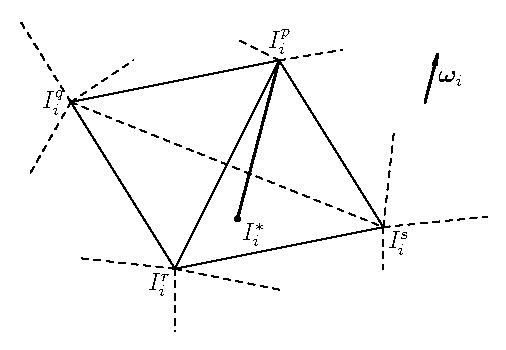
\includegraphics[height=.2\textheight]{radiation-2.eps}
\caption{Схема сеточно-характеристического метода}
\label{fig:char}
\end{figure}

Простейшим представителем конечно-объёмных методов является метод Годунова. В основе конечно-объемных методов лежат интегральные законы сохранения. Проинтегрируем уравнение переноса
\eqref{eq:grid} по объему тетраэдра $T$ (для краткости будем опускать индекс направления $i$):
\[
\int\limits_T \div (\vec \omega I(\vec r))  d\vec r + \int\limits_T \varkappa(\vec r) I(\vec r)  d\vec r = \int\limits_T \varkappa(\vec r) I_\text{p}(\vec r)  d\vec r.
\]
Интеграл от дивергенции может быть записан в виде интеграла по границе:
\[
\int\limits_T \div (\vec \omega I(\vec r)) d\vec r= \int_{\partial T} \vec n \vec \omega I(\vec r) d\Gamma.
\]
В конечно-объемных методах нормальный поток на границе конечного объема определяется из точного либо приближенного решения задачи Римана о распаде разрыва \cite{Kulikovskiy2001}.
Для уравнения переноса излучения задача Римана имеет простое решение. Пусть значение интенсивности излучения в полупространстве $\vec r \vec n < 0$ равно $I_L$, а значение в полупространстве $\vec r \vec n > 0$ равно $I_R$. Тогда поток интенсивности излучения $\vec \omega I$ через границу $\vec r \vec n = 0$ равен
\[
\vec \omega I\big|_{\vec r \vec n = 0} = 
\begin{cases}
\vec \omega I_L, &\vec \omega \vec n > 0\\
\vec \omega I_R, &\vec \omega \vec n \leq 0
\end{cases}.
\] 
Заметим, что отнесение $\vec \omega \vec n = 0$ к одному из этих случаев несущественно, так как нормальный поток в любом случае будет равен нулю.

Назовем грань $f_j$ тэтраэдра $T$ \emph{входной}, если внешняя нормаль $\vec n_j$ составляет с направлением изучения $\vec \omega$ тупой угол, и \emph{выходной} в противном случае.
Примем гипотезу о постоянном распределении величин $I, \varkappa, I_{\text{p}}$ в тетраэдре $T$. Обозначим $I^0$ интенсивность излучения в тетраэдре $T$, а $I^j$ --- интенсивность излучения в тетраэдре, граничащем с $T$ по грани $f_j$. Используя выражение для нормального потока из решения задачи Римана, получаем метод Годунова для уравнения переноса излучения:
\begin{equation}
\frac{1}{V(T)}\left[
\sum_{\substack{f_j \in \partial T\\\vec n_j \vec \omega < 0}} \vec S_j \vec \omega I^j 
+
\sum_{\substack{f_j \in \partial T\\\vec n_j \vec \omega > 0}} \vec S_j \vec \omega I^0
\right]
+ \varkappa I^0 = \varkappa I_\text{p},
\label{eq:fvm}
\end{equation}
где посредством $\vec S_j$обозначена векторная площадь грани $j$, то есть площадь, умноженная на внешнюю нормаль $\vec n_j$, а $V(T)$ --- объём тетраэдра $T$. Можно видеть, что для определения $I^0$ необходимо знать интенсивность излучения $I^j$ во всех тетраэдрах, граничащих с $T$ по его входным граням.

Разностные задачи, полученные либо сеточно-характеристичекими, либо конечно-объёмными методами, представляют собой набор линейных уравнений относительно неизвестных значений интенсивности. Данные уравнения можно решить итерационно, например методом установления, фактически превратив исходную стационарную гиперболическую задачу в нестрационарную. Однако, эти задачи могут быть решены и безытерационным методами, в которых решение строится последовательным обходом неизвестных (маршем), при котором для вычисления очередной неизвестной все необходимые данные были найдены раньше.
Данные методы имеют преимущество, так как требуют лишь однократного прохода по расчетной области, в отличие от итерационных методов, в которых необходимо многократно повторять вычисления для каждого узла до достижения требуемой точности.

\section{Метод коротких характеристик второго порядка аппроксимации}

Рассмотрим метод коротких характеристик, в котором интенсивность излучения задана в нескольких узлах на гранях тетраэдров, но без конкретизации расположения данных узлов и их количества. Будем предполагать, что коэффициенты поглощения и интенсивность равновесного излучения постоянны в каждом тетраэдре.

Для определения решения на грани требуется определить решение в каждом узле, расположенном на данной грани. Для этого из каждого узла грани выпускается характеристика в направлении $-\vec\omega$ до пересечения с гранью тетраэдра (см. рисунок \ref{fig:manychar}). Заметим, что эта грань будет входной, так как характеристика выходит из тетраэдра в направлении $-\vec\omega$ под острым углом к нормали $\vec n$ к грани. Различные характеристики могут выходить из тетраэдра через различные входные грани, поэтому до вычисления решения на выходной грани, все входные грани должны быть уже освещены (то есть, решение на них уже должно быть найдено).
\begin{figure}[ht!]
\centering
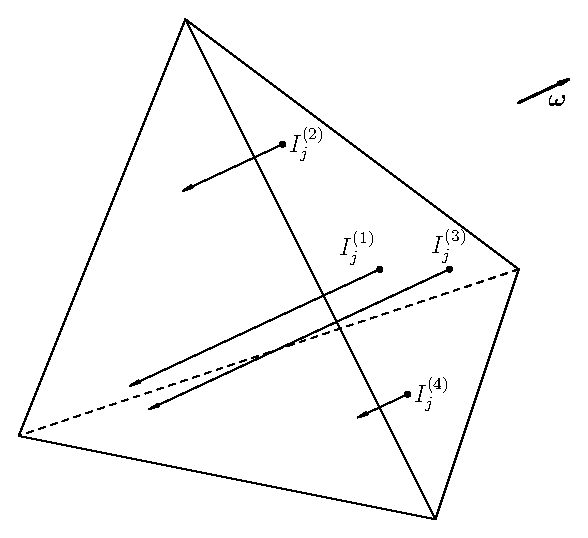
\includegraphics[height=.3\textheight]{radiation-4.eps}
\caption{Характеристики, выпущенные из нескольких узлов на грани тетраэдра}
\label{fig:manychar}
\end{figure}

Вдоль каждой характеристики уравнение переноса является обыкновенным дифференциальным уравнением
\[
\frac{dI}{ds} + \varkappa I = \varkappa I_\text{p},
\]
причем величины $\varkappa$ и $I_\text{p}$ постоянны по предположению. Решение этого уравнения может быть записано в виде
\begin{equation}
I = e^{-\tau} I^*  + \left(1 - e^{-\tau}\right) I_\text{p},
\label{eq:shortchar}
\end{equation}
где $I$ --- интенсивность излучения в точке, из которой выпускается характеристика, $I^*$ --- интенсивность излучения в точке пересечения характеристики с входной гранью, а $\tau$ --- оптическая длина характеристики, равная ее длине $\ell$, умноженной на коэффициент поглощения $\varkappa$. Из \eqref{eq:shortchar} следует, что интенсивность $I$ не выходит за диапазон значений $[\min(I^*, I_\text{p}), \max(I^*, I_\text{p})]$.

Величина $I^*$ определяется интерполяцией по значениям интенсивности в узлах той грани, через которую выходит характеристика. Порядок аппроксимации метода соответствует степени используемой интерполяции. Для получения метода второго порядка необходимо пользоваться квадратичной интерполяцией значений интенсивности на грани, при этом необходимо знать значение интенсивности в шести узлах на данной грани.

Повысить порядок метода можно и не увеличивая количество узлов на грани, а пользуясь значениями интенсивности на соседних гранях. Однако, данный способ увеличивает разностный шаблон, нарушая компактность схемы. При расширении шаблона появляются дополнительные зависимости между решением на различных гранях, что существенно осложняет алгоритм упорядочения неизвестных.

Таким образом, для построения метода второго порядка необходимо на каждой грани выбрать шесть узлов интерполяции.

\subsection{Расположение узловых точек}

Расположение узлов интерполяции на грани не может быть произвольным. Применим данный метод к двумерному уравнению переноса излучения на равномерной прямоугольной сетке. Ограничимся методом первого порядка. На каждой грани (которая в двумерном случае является просто отрезком) возьмем два узла для линейной интерполяции, но расположим их строго внутри грани (см. рисунок \ref{fig:instab}).

В случае, когда излучение распространяется под малым углом к вертикали $\omega_x < \sin \theta_\text{кр}$, численное решение переносится только вертикально, при этом нарушается необходимое условие устойчивости разностного метода: область зависимости численного решения не содержит область зависимости решения дифференциальной задачи. Пусть $I_j^{(1)}$ и $I_j^{(2)}$ --- значения интенсивности соответственно в левом и правом узле на $j$-ом слое в некотором фиксированном столбце. Тогда в простейшем случае $\varkappa = 0, I_\text{p} = 0$ численное решение удовлетворяет соотношениям
\begin{gather*}
I_{j+1}^{(1)} = I_{j}^{(1)} - \frac{\omega_x}{\omega_y} \frac{I_{j}^{(2)} - I_{j}^{(1)}}{1 - 2\tg \theta_\text{кр}},\\
I_{j+1}^{(2)} = I_{j}^{(2)} - \frac{\omega_x}{\omega_y} \frac{I_{j}^{(2)} - I_{j}^{(1)}}{1 - 2\tg \theta_\text{кр}}.
\end{gather*}
В зависимости от знака $I_0^{(2)} - I_0^{(1)}$ решение $I_j^{(1,2)}$ неограниченно стремится либо к $+\infty$, либо к $-\infty$.

\begin{figure}[ht!]
\centering
\includegraphics[height=.35\textheight]{instab-0.eps}
\caption{Направление распространения излучения в численной схеме (контурная стрелка) и истинное направление $\vec \omega$}
\label{fig:instab}
\end{figure}

Данный эффект не возможен, если узлы располагать в вершинах сетки. При этом $\theta_\text{кр} = 0$. По данной причине в методе второго порядка узлы на гранях обязательно должны содержать 
вершины грани. Расположение остальных трех узлов может быть произвольно, но для простоты эти узлы были взяты на ребрах грани.

\subsection{Монотонизация схемы}

Как известно из теоремы Годунова, никакая линейная схема выше первого порядка не может быть монотонной. Немонотонность схемы второго порядка может приводить к нарушению выполнения принципа максимума, а также появлению нефизических (отрицательных) значений интенсивности. Из \eqref{eq:shortchar} следует, что процедура интегрирования вдоль характеристики является монотонной, а немонотонность может быть вызвана только интерполяцией интенсивности по грани.

Рассмотрим треугольную грань $T$ и квадратичную форму $I(\vec \xi)$ на ней. Чтобы форма была монотонной на грани $T$ необходимо, чтобы на всех ребрах грани $T$ форма была монотонна.
Если $I_1$ и $I_2$ --- значения формы на концах ребра, а $I_\text{ц}$ --- значение формы в середине ребра, то квадратичная форма на ребре имеет вид
\[
I(t) = I_\text{ц} + \frac{I_2 - I_1}{2} t + \frac{I_1 -2 I_\text{ц} + I_2}{2} t^2,
\]
где $t$ --- координата вдоль ребра, принимающая в концах ребра значения $\pm 1$. Эта форма не будет иметь экстремумов на интервале $t \in (-1, 1)$ при выполнении условия
\[
\left|\frac{I_2 - I_1}{2}\right| \geq |I_1 -2 I_\text{ц} + I_2|,
\]
что также можно записать в виде
\begin{equation}
\left|I_\text{ц} - \frac{I_1 + I_2}{2}\right| \leq \frac{|I_2 - I_1|}{4}.
\label{eq:mono}
\end{equation}
При выполнении этого условия максимум и минимум квадратичной формы $I(\vec \xi)$ по границе $\partial T$ достигается в вершинах треугольника $T$. Таким образом, если квадратичная форма $I(\vec \xi)$ имеет на треугольнике $T$ значения, выходящие за пределы значений в вершинах, то это может произойти лишь строго внутри треугольника. Иными словами, внутри треугольника должен находиться экстремум квадратичной формы $I(\vec \xi)$. Но при этом некоторые линии уровня $I(\vec \xi) = 0$ будут касаться сторон треугольника (см. рисунок \ref{fig:extr}), что означает существование локального экстремума квадратичной формы на ребре. Но это невозможно, а следовательно, квадратичная форма не может иметь локальных экстремумов внутри треугольника и является в нем монотонной.
\begin{figure}[ht!]
\centering

\includegraphics[height=.25\textheight]{extr-1.eps}
\caption{Линии уровня квадратичной формы при наличии экстремума внутри треугольника}
\label{fig:extr}
\end{figure}

Таким образом, условие монотонности \eqref{eq:mono} формы на ребрах является необходимым и достаточным для монотонности на всем треугольнике. Обеспечить его выполнение можно коррекцией значения в центре ребра $I_\text{ц}$:
\[
I_\text{ц}^\text{корр} = 
\frac{I_1 + I_2}{2} + \operatorname{clamp}\left(
I_\text{ц} - \frac{I_1 + I_2}{2}, 
\left[
-\frac{|I_2 - I_1|}{4},
\frac{|I_2 - I_1|}{4}
\right]
\right),
\]
где функция $\operatorname{clamp}(x, [a, b])$ <<зажимает>> значение $x$ в пределах отрезка $[a, b]$ и определяется как
\[
\operatorname{clamp}(x, [a, b]) = \max(a, \min(b, x)).
\]

Можно видеть, что метод второго порядка с данным ограничителем не хуже метода первого порядка, так как метод первого порядка получается при ограничении по правилу
\[
I_\text{ц}^\text{корр} = \frac{I_1 + I_2}{2}.
\]

\section{Алгоритмы упорядочения сеточных элементов}

Выше было показано, что как сеточно-характеристические, так и конечно-объемные схемы допускают построение численного решения маршевым образом. Для этого необходимо ввести порядок, в котором вычисляется решение по граням тетраэдров. Будем говорить, что тетраэдр $T$ следует за тетраэдром $T'$ ($T \succ T'$) если их общая грань является выходной для $T'$ и входной для $T$. В конечно-объемных методах решение в тетраэдре $T$ можно вычислить тогда, когда решения во всех предшествующих ему тетраэдрах $T' \prec T$ уже вычислены. В сеточно-характеристических методах вычисление решения в тетраэдре $T$ можно отождествить с вычислением решения на всех его выходных гранях, при этом необходимо знать решение на всех входных гранях, что соответствует нахождению решения во всех предшествующих ему тетраэдрах $T' \prec T$. Таким образом, упорядочение тетраэдров относительно отношения $T' \prec T$ является основой маршевого алгоритма как для сеточно-характеристических, так и для конечно-объемного методов.

Граф, связанный с отношением $\succ$, является ориентированным. Назовем упорядочением графа такую нумерацию тетраэдров $c(T)$ такую, что \[c(T) < c(T') \Leftrightarrow T \prec T'.\]
Нумерация не обязана быть инъективной, то есть из $c(T) = c(T')$ не обязано следовать, что $T = T'$.
Очевидно, что если в графе есть цикл
\[
T \prec T' \prec \dots \prec T'' \prec T,
\]
то упорядочение невозможно в силу $c(T) < \dots < c(T)$. Будем предполагать, что граф, связанный с отношением $\succ$ является направленным ациклическим графом. Известно \cite{Kahn1962}, что направленный ациклический граф всегда можно упорядочить.

\subsection{Алгоритм для триангуляций Делоне}

Предположим, что триангуляция области удовлетворяет условию Делоне, то есть для каждого тетраэдра $T$ в его описанной сфере не содержится целиком никакой другой тетраэдр $T'$.
Пусть $\pi(T) = \vec \omega \vec r_c(T)$, где $\vec r_c(T)$ --- радиус вектор центра описанной вокруг $T$ сферы, $\vec \omega$ --- направление излучения. Тогда сортировка тетраэдров по возрастанию значения $\pi(T)$ дает необходимый порядок $c(T)$, то есть $T \prec T' \Rightarrow \pi(T) < \pi(T')$ \cite{skalko2014}.

Докажем данное утверждение. Предположим, что для некоторой пары $T \succ T'$ выполняется $\pi(T) < \pi(T')$. Пусть $O, O'$ --- центры описанных вокруг $T, T'$ сфер (см. рисунок \ref{fig:spheres}). Пусть для определенности нормаль $\vec n$ направлена внутрь тетраэдра $T$. Тогда вектор $\overrightarrow{OO'}$ коллинеарен с вектором нормали $\vec n$ к грани, общей для $T, T'$. Пусть $V, V'$ --- вершины, противоположные этой грани в тетраэдрах $T, T'$. Тогда $\overrightarrow{V'V} \vec n > 0$. Действительно, пусть $M$ --- произвольная точка грани. Объёмы тетраэдров $T, T'$ равны
\begin{figure}[ht!]
\centering
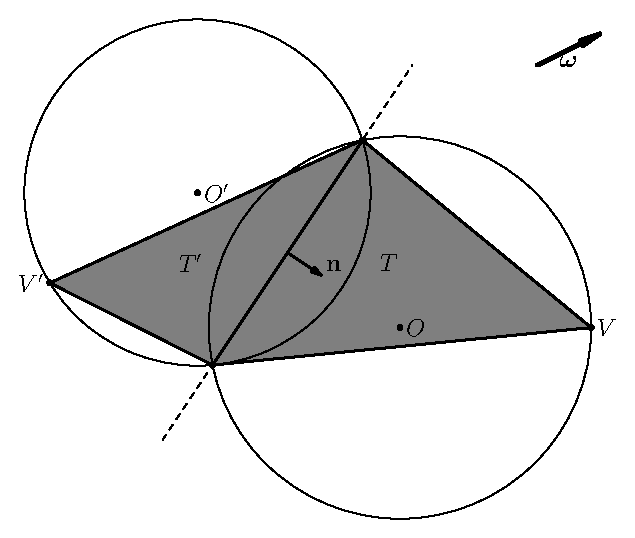
\includegraphics[height=.35\textheight]{spheres-0.eps}
\caption{К доказательству корректности упорядочения для триангуляций Делоне}
\label{fig:spheres}
\end{figure}
\[
V(T) = \frac{1}{3} S \vec n \overrightarrow{MV}, \qquad V(T') = \frac{1}{3} S \vec n \overrightarrow{V'M},
\]
где $S$ --- площадь их общей грани. Суммируя и учитывая $V(T) + V(T') > 0$, получаем
\[
\vec n \overrightarrow{V'V} > 0.
\]

Условие Делоне означает, что расстояние от точки $O$ до $V'$ должно быть больше расстояния от $O$ до $V$. Аналогично для второй сферы:
\[
|OV'| > |OV|, \quad |O'V| > |O'V'|.
\]
Возводя последние соотношения в квадрат, получаем
\[
(\overrightarrow{OV'},\overrightarrow{OV'}) - (\overrightarrow{OV},\overrightarrow{OV}) > 0, \qquad
(\overrightarrow{O'V},\overrightarrow{O'V}) - (\overrightarrow{O'V'},\overrightarrow{O'V'}) > 0
\]
Добавляя и вычитая $(\overrightarrow{OV'},\overrightarrow{OV})$, получаем
\begin{multline*}
0 < (\overrightarrow{OV'},\overrightarrow{OV'}) - (\overrightarrow{OV},\overrightarrow{OV}) =
(\overrightarrow{OV'},\overrightarrow{OV'}) 
-(\overrightarrow{OV'},\overrightarrow{OV})
+(\overrightarrow{OV'},\overrightarrow{OV})
- (\overrightarrow{OV},\overrightarrow{OV}) = \\ =
(\overrightarrow{OV'},\overrightarrow{VV'}) 
+
(\overrightarrow{VV'}, \overrightarrow{OV}) = 
\left(\overrightarrow{VV'}, \frac{\overrightarrow{OV}+ \overrightarrow{OV'}}{2}\right)
\end{multline*}
Аналогично,
\[
\left(\overrightarrow{V'V}, \frac{\overrightarrow{O'V}+ \overrightarrow{O'V'}}{2}\right)  =
\left(\overrightarrow{VV'}, \frac{\overrightarrow{VO'}+ \overrightarrow{V'O'}}{2}\right) 
> 0.
\]
Суммируя данные неравенства, получаем
\begin{equation}
(\overrightarrow{VV'},\overrightarrow{OO'}) > 0.
\label{eq:half}
\end{equation}
Так как точки $O,O'$ (а также $V,V'$) находятся в разных полупространствах, разделенных гранью, условие \eqref{eq:half} показывает, что точки $O$ и $V$ находятся с одной стороны грани, а $O'$ и $V'$ --- с другой. Таким образом, вектор $\overrightarrow{O'O}$ не только коллинеарен $\vec n$, но и сонаправлен с ним. Поэтому условие $T \succ T'$, эквивалентное $\vec \omega \vec n > 0$, эквивалентно $\vec \omega \overrightarrow{O'O} > 0$, что в свою очередь эквивалентно $\pi(T) > \pi(T')$. Полученное противоречие доказывает $T \prec T' \Rightarrow \pi(T) < \pi(T')$.

Используемые строгие неравенства предполагают общее расположение тераэдров (описанные сферы двух тетраэдров не могут совпадать). Выполнения этого условия можно добиться небольшим возмущением триангуляции. Заметим, что для триангуляции Делоне невозможно образование циклов в отношении $\prec$.


\subsection{Алгоритм для триангуляций общего вида}

Для построения упорядочения $c(T)$ триангуляции общего вида можно воспользоваться модификацией алгоритма Тарьяна \cite{Corman2009} для топологической сортировки, который в свою очередь, является простой модификацией поиска в ширину.

В алгоритме \ref{alg:coloring} используется очередь тетраэдров, заполненная изначально тетраэдрами, у которых все входные грани освещены, то есть теми тетраэдрами, для которых на всех входных гранях задано граничное условие.

На очередном шаге алгоритма из очереди извлекается тетраэдр $T$. Проверяется, присвоен ли номер $c(T_j)$ всем его предшествующим соседям $T_j \prec T$. Если это так, тетраэдру $T$ присваивается номер
\[
c(T) = 1 + \max_{T_j \prec T} c(T_j).
\]
В случае, когда тетраэдр $T$ лежит на границе области, для отсутствующих соседей $T_j$ формально полагается $c(T_j) = 0$. Это позволяет присвоить всем тетраэдрам, которые изначально были в очереди номер $c(T) = 1$. После присвоения номера тетраэдру $T$, в очередь добавляются все следующие за ним тетраэдры $T' \succ T$, которым еще не присвоен номер.

Если хотя бы одному предшествующему соседу $T_j \prec T$ еще не присвоен номер, тетраэдр $T$ возвращается в конец очереди. Данный алгоритм способен определять наличие циклов в отношении $\prec$. Если в триангуляции обнаружен цикл, тетраэдры будут постоянно извлекаться и добавляться в конец очереди. Алгоритмически это можно определить используя счетчик. После добавления нового тетраэдра в очередь счетчик устанавливается равным длине очереди, а при возвращении тетраэдра обратно в очередь, счетчик уменьшается на единицу. Если на очередном шаге алгоритма счетчик обнуляется, это свидетельствует о том, что последние $n$ шагов алгоритма из очереди длины $n$ тетраэдры только извлекались и добавлялись обратно, причем ни одному новому тетраэдру не был присвоен номер. Данный факт свидетельствует о зацикливании алгоритма, а значит граф отношения $\prec$ не является ациклическим. Работа алгоритма проиллюстрирована на рисунке \ref{fig:coloring}.
\begin{figure}[ht!]
\centering
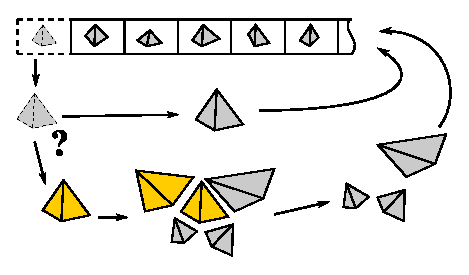
\includegraphics[height=.2\textheight]{coloring.eps}
\caption{Иллюстрация работы алгоритма упорядочения}
\label{fig:coloring}
\end{figure}

\begin{algorithm}[ht!]
\centering
\begin{algorithmic}[1]
\Procedure{Ordering}{}
\State $Q :=$ \Call{InitQueue}{}
\State $cnt := |Q|$
\While {$Q \neq \emptyset$}
\State $T :=$ \Call{Dequeue}{$Q$}
\If {$\forall T' \prec T, c(T') \neq \mathbf{nil}$}
\State $c(T) := 1 + \max_{T' \prec T} c(T')$
\For {$T'' \succ T: c(T'') = \mathbf{nil}$}
\State \Call{Enqueue}{$Q$, $T''$}
\EndFor
\State $cnt := |Q|$
\Else
\State \Call{Enqueue}{$Q$, $T$}
\State $cnt := cnt - 1$;
\EndIf
\If {$cnt < 0$}
\State \textbf{error} В триангуляции обнаружен цикл.
\EndIf
\EndWhile
\EndProcedure
\end{algorithmic}
\caption{Алгоритм упорядочения для произвольной триангуляции}
\label{alg:coloring}
\end{algorithm}

Заметим, что данное упорядочение является оптимальным в том смысле, что каждому тетраэдру $T$ присваивается минимально возможный номер $c(T)$. При этом максимальный номер будет присвоен последнему тетраэдру в самой длинной цепочке зависимых тетраэдров
\[
T_1 \prec T_2 \prec \dots \prec T_n.
\]

\section{Связь минимального порядка $c(T)$ с ярусно-параллельной формой алгоритма}

Если упорядочение $c(T)$ минимально, например, построено с помощью алгоритма \ref{alg:coloring}, то множество всех тетраэдров сетки разбивается на непересекающиеся подмножества
\[
U_k = \left\{T \mid c(T) = k\right\}.
\]
При этом для вычисления решения в каждом тетраэдре $T \in U_k$ достаточно знать решения для каждого тетраэдра $T' \in \bigcup_{j = 1}^{k - 1} U_j$. В частности, решение в $T$ не зависит от решения в тетраэдрах $T''$ с тем же номером $c(T'') = k$. Последнее свойство означает, что решения во всех тетраэдрах из $U_k$ можно находить параллельно.

Заметим, что ациклический граф отношения $\prec$ является также графом зависимостей вычислительного алгоритма, а построенное упорядочение фактически задает ярусно-параллельную его форму \cite{Karpov2014}. По определению, ярусно-параллельной формой называется деление графа на такие множества $V_i$, что для каждой дуги $u \to v, u \in V_j, v \in V_k$ выполняется $j < k$.
В маршевом методе решение вычисляется последовательно для каждого множества $U_k, k = 1, \dots, n$, но в каждом множестве $U_k$ решение может вычисляться параллельно. На рисунке \ref{fig:marching} показаны тетраэдры, в которых решение уже вычислено для различных моментов <<марша>>: в начале, в середине и в конце.

\begin{figure}[ht!]
\centering
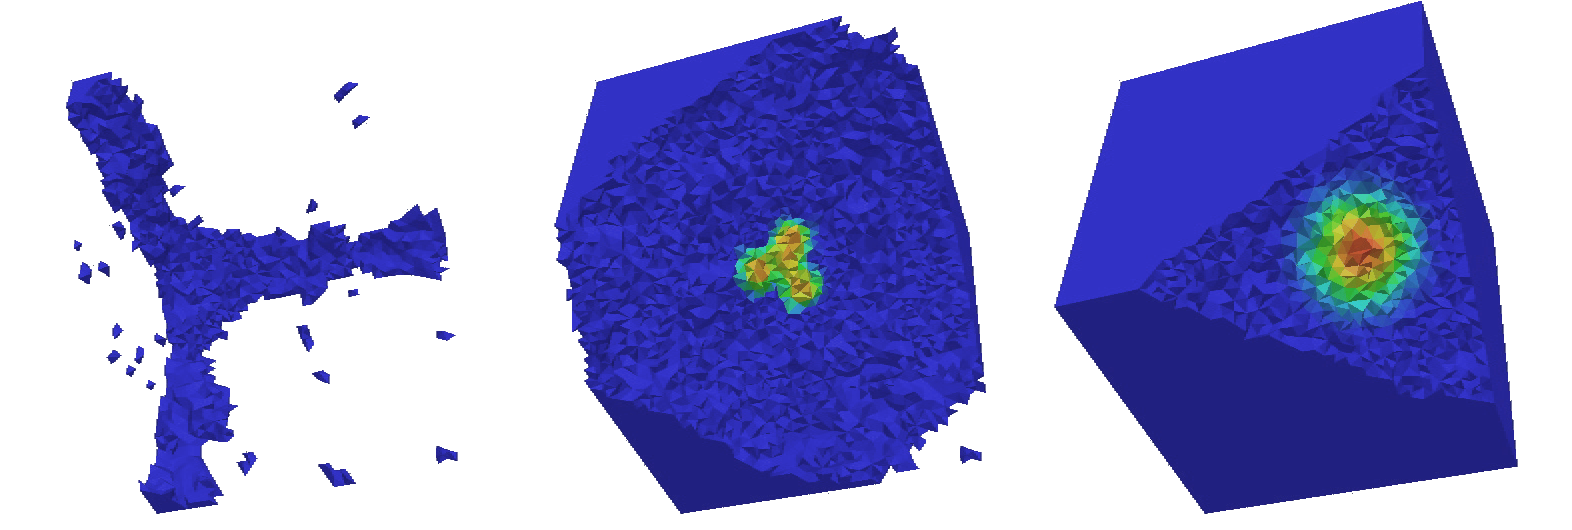
\includegraphics[height=.2\textheight]{123.png}
\caption{Множество тетраэдров с номером $c(T) < k$ для различных $k$}
\label{fig:marching}
\end{figure}

Однако, для параллельной реализации алгоритма требуется учитывать накладные расходы на построение упорядочения $c(T)$. Алгоритм упорядочения существенно последователен, поэтому выигрыш от распараллеливания возможен лишь в двух случаях
\begin{itemize}
\item решение задачи в каждом тетраэдре ресурсоемко, например, одновременно решается уравнение переноса для большого числа частот;
\item производится многократное решение уравнения переноса, например, на протяжении большого числа шагов по времени.
\end{itemize}
В последнем случае для каждого направления переноса необходимо хранить упорядочение $c(T)$. К тому же, между шагами по времени не должна изменяться расчетная сетка. Последнее обстоятельство сильно ограничивает применимость параллельного алгоритма на подвижных сетках.           % Глава 3
\chapter{Распределенный метод длинных характеристик}

Метод длинных характеристик является наиболее точным методом решения уравнения переноса излучения. Метод основывается на точном решении уравнения переноса в каждом направлении.

Уравнение переноса 
\[
(\vec \Omega \nabla) I(\vec r, \vec \Omega) + \varkappa(\vec r, \vec \Omega) I(\vec r, \vec \Omega) = \varkappa(\vec r, \vec \Omega) I_\text{p}(\vec r, \vec \Omega)
\]
вдоль характеристики
$
\vec r - \vec r_0 = \vec \Omega (s - s_0)
$
превращается в обыкновенное дифференциальное уравнение
\[
\frac{dI(s)}{ds} + \varkappa(s) I(s) = \varkappa(s) I_\text{p}(s)
\]
и может быть легко проинтегрировано точно:
\begin{equation}
I(s) = I(s_0) e^{-\tau(s_0, s)} + \int_{s_0}^s \varkappa(\xi) I_\text{p}(\xi)
e^{-\tau(\xi,s)} d\xi.
\label{eq:exact}
\end{equation}
В последнем выражении $\tau(a,b) = \int_a^b \varkappa(s) ds$ --- оптическая длина отрезка характеристики от точки $s = a$ до точки $s = b$.

Соотношение \eqref{eq:exact} лежит в основе метода длинных характеристик. В отличие от метода коротких характеристик, где характеристика выпускается из узла до входной грани тетраэдра, в методе длинных характеристик она выпускается до границы расчетной области, см. рисунок \ref{fig:lcm}.
\begin{figure}[ht!]
\centering
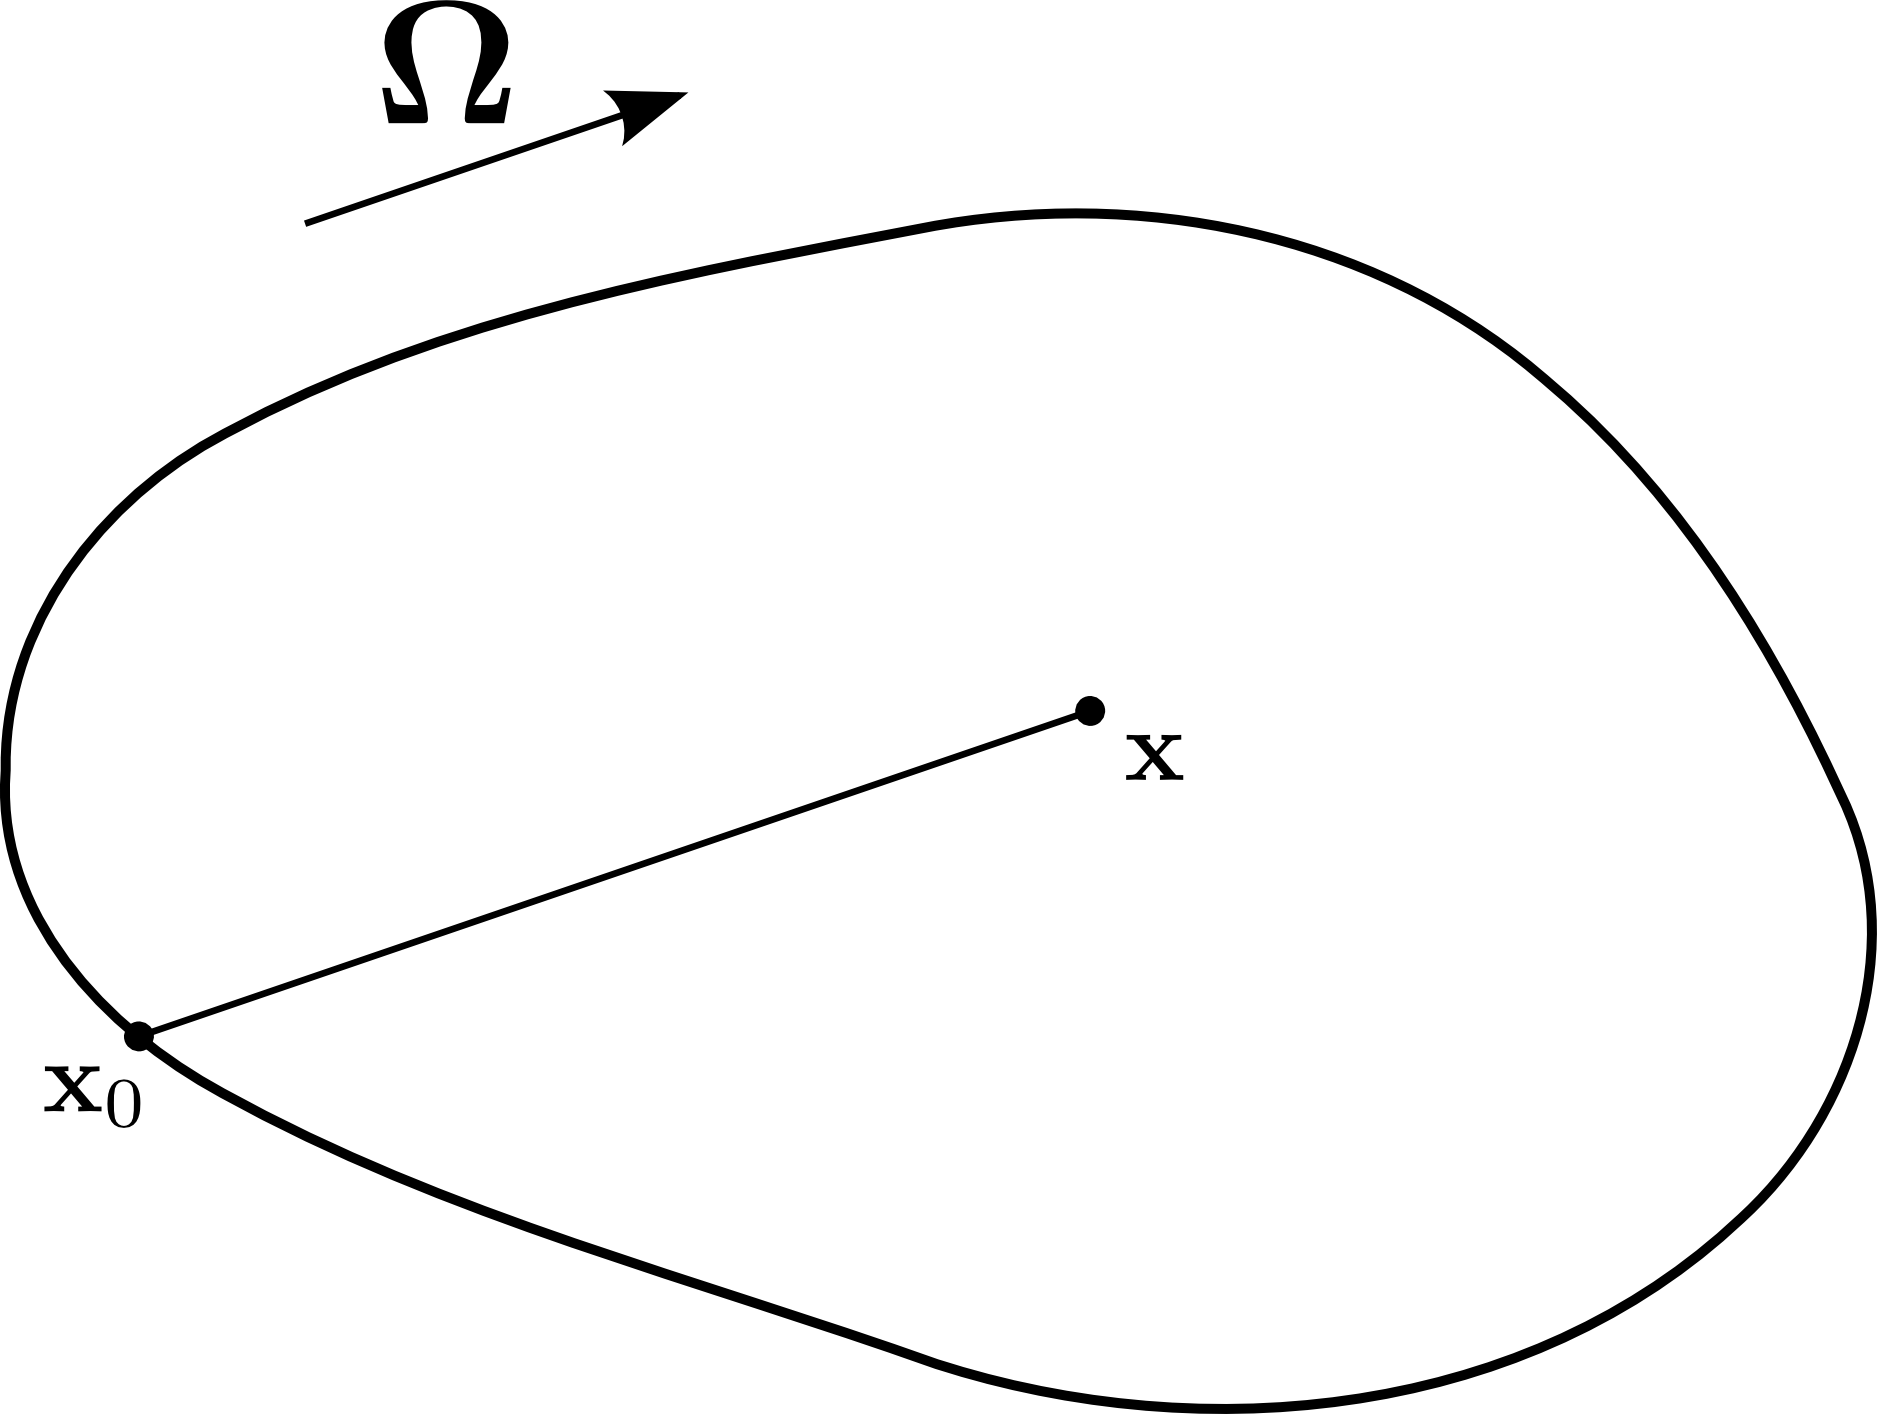
\includegraphics[height=0.25\textheight]{lcm.png}
\caption{Нахождение решения методом длинных характеристик}
\label{fig:lcm}
\end{figure}

\section{Функция Грина для задачи переноса излучения}

Заметим, что соотношение \eqref{eq:exact} представляет собой выражение функции Грина, так как связывает решение в точке $I(\vec r, \vec \Omega)$ с граничным условием $I(\vec r_0, \vec \Omega), \vec r_0 \in \partial G$.

Введем обозначения $\alpha(s_0, s)$ и $\beta(s_0, s)$ 
\begin{gather*}
\alpha(s_0, s) = e^{-\tau(s_0, s)}\\
\beta(s_0, s) = \int\limits_{s_0}^s \varkappa(\xi) I_\text{p}(\xi) \alpha(\xi, s) d\xi.
\end{gather*}

В этих обозначениях функция Грина записывается в виде
\begin{equation}
I(s) = \alpha(s_0, s) I(s_0) + \beta(s_0, s).
\label{eq:connection}
\end{equation}
При $s > s_0$ для величин $\alpha(s_0, s), \beta(s_0, s)$ справедливо
\begin{equation}
\begin{gathered}
0 < \alpha(s_0, s) \leqslant 1\\
0 \leqslant \beta(s_0, s) \leqslant \max_{\xi \in [s_0, s]} I_\text{p}(\xi)
\cdot \int_{s_0}^s \varkappa(\xi) e^{-\tau(\xi, s)} d\xi = \\ =
\max_{\xi \in [s_0, s]} I_\text{p}(\xi)
\cdot \int_{0}^{\tau(s_0,s)} e^{-u} du =
(1 - \alpha(s_0, s))\max_{\xi \in [s_0, s]} I_\text{p}(\xi).
\end{gathered}
\label{eq:limits}
\end{equation}
С учетом \eqref{eq:limits} для $I(s)$ верен принцип максимума
\[
I(s) \leqslant \alpha(s_0, s) I(s_0) + (1 - \alpha(s_0, s))\max_{\xi \in [s_0, s]} I_\text{p}(\xi) \leqslant \max\left(I(s_0); \max_{\xi \in [s_0, s]} I_\text{p}(\xi)\right).
\]

Фактически, функция Грина задается лишь двумя коэффициентами для каждой точки $\vec r$ и направления $\vec \Omega$. В численном методе точка $\vec r_0$ не является узлом сетки, а значение $I(\vec r_0, \vec \Omega)$ находится интерполяцией интенсивности по грани, содержащей точку $\vec r_0$. При этом численная функция Грина дополнительно задается коэффициентами интерполяции и номерами вершин грани.

Для сравнения, численная функция Грина, построенная в методе коротких характеристик, зависит от большого числа узлов на границе. Увеличение шаблона вызвано в этом методе многократной интерполяцией.

\subsection{Трассировочное соотношение}

Для практического вычисления коэффициентов $\alpha(s_0, s)$ и $\beta(s_0, s)$ удобно пользоваться следующим соотношением при $s_0 \leq s_1 \leq s$:
\[
\alpha(s_0, s) = e^{-\tau(s_0, s)} = 
e^{-\tau(s_0, s_1) -\tau(s_1, s)} = 
\alpha(s_0, s_1)\alpha(s_1, s),
\]
следующим из аддитивности оптической длины.

Для $\beta(s_0, s)$ справедливо
\begin{multline*}
\beta(s_0, s) = 
\int\limits_{s_0}^s \varkappa(\xi) I_\text{p}(\xi) \alpha(\xi, s) d\xi = \\ =
\int\limits_{s_0}^{s_1} \varkappa(\xi) I_\text{p}(\xi) \alpha(\xi, s) d\xi +
\int\limits_{s_1}^s \varkappa(\xi) I_\text{p}(\xi) \alpha(\xi, s) d\xi = \\ =
\int\limits_{s_0}^{s_1} \varkappa(\xi) I_\text{p}(\xi) \alpha(\xi, s_1) \alpha(s_1, s) d\xi +
\int\limits_{s_1}^s \varkappa(\xi) I_\text{p}(\xi) \alpha(\xi, s) d\xi = \\
= \beta(s_0, s_1) \alpha(s_1, s) + \beta(s_1, s).
\end{multline*}

Фактически, соотношения между коэффициентами $\alpha, \beta$ следуют из принципа Гюйгенса
\begin{multline*}
I(s) = \alpha(s_1, s) I(s_1) + \beta(s_1, s) = \\ =
\alpha(s_1, s) \Big(\alpha(s_0, s_1) I(s_0) + \beta(s_0, s_1)\Big) + \beta(s_1, s)
= \\ =
\alpha(s_0, s_1)\alpha(s_1, s) I(s_0) + \beta(s_0, s_1)\alpha(s_1, s) + \beta(s_1, s).
\end{multline*}

Будем называть соотношения
\begin{equation}
\begin{gathered}
\alpha(s_0, s) = \alpha(s_0, s_1)\alpha(s_1, s),\\
\beta(s_0, s) = \beta(s_0, s_1) \alpha(s_1, s) + \beta(s_1, s)
\end{gathered}
\end{equation}
трассировочными. С помощью них удобно вычислять коэффициенты $\alpha(s_0, s), \beta(s_0, s)$, двигаясь вдоль характеристики по тетраэдрам триангуляции (см. рисунок \ref{fig:trace}). При переходе от коэффициентов $\alpha(s_1, s), \beta(s_1, s)$ к коэффициентам $\alpha(s_0, s), \beta(s_0, s)$ достаточно знать только значения
$\alpha(s_0, s_1), \beta(s_0, s_1)$. Для однородных значений $\varkappa, I_\text{p}$ в тетраэдре,
\[
\alpha(s_0, s_1) = e^{-\varkappa (s_1 - s_0)},\qquad
\beta(s_0, s_1) = \big(1 - \alpha(s_0, s_1)\big) I_\text{p}.
\]
\begin{figure}[ht!]
\centering
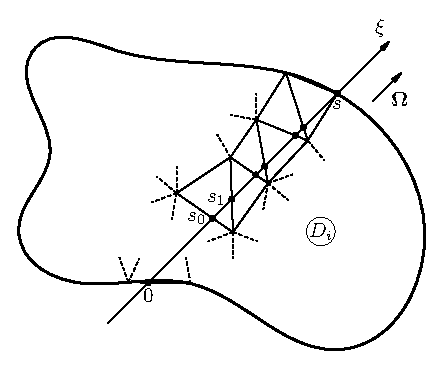
\includegraphics[width=.4\textwidth]{trace-0.eps}
\caption{Трассировка луча по триангуляции}
\label{fig:trace}
\end{figure}

\section{Устойчивая трассировки луча}

Рассмотрим процесс трассировки луча из точки $\vec r$. Трассировка начинается в тетраэдре $T$, содержащем точку $\vec r - 0 \vec \Omega$. Для каждой треугольной грани $Q = \operatorname{conv}(r_1, r_2, r_3)$ тетраэдра находятся барицентрические координаты $\gamma_k$ точки пересечения $\vec r^* = \sum_{k=1}^3 \gamma_k \vec r_k$ плоскости грани с лучом $\vec r - \vec \Omega s$.  Находится грань, для которой все барицентрические координаты $\gamma_k$ неотрицательны. Для этой грани $\vec r^* \in Q$. Псевдокод данной процедуры изложен в алгоритме \ref{alg:traceelem}  
\begin{algorithm}[ht!]
\centering
\begin{algorithmic}[1]
\Function{TraceElement}{$e$, $P \in e, \vec \omega$}
%\State $P := $ \Call{ShiftToStable}{$e, P$}
\For{каждой грани $f \in e$}
\State $(\vec r_1, \vec r_2, \vec r_3) := $ \Call{VertexCoordinates}{$f$}
\State $\triangleright$  Решить
$(
\vec r_P - \ell \vec \omega - \vec r_1,
\vec r_2 - \vec r_1,
\vec r_3 - \vec r_1
) = 0$ относительно $\ell$
\If{$(\vec \omega, \vec r_2 - \vec r_1, \vec r_3 - \vec r_1) = 0$}
\State $\mu(f) := \infty$
\State \textbf{continue} \Comment Перейти к следующей грани
\EndIf
\State $\ell := 
\dfrac{(\vec r_P - \vec r_1, \vec r_2 - \vec r_1, \vec r_3 - \vec r_1)}
{(\vec \omega, \vec r_2 - \vec r_1, \vec r_3 - \vec r_1)}$
\If{$\ell < 0$}
\State $\mu(f) := \infty$
\State \textbf{continue} \Comment Перейти к следующей грани
\EndIf
\State $\vec r_Q := \vec r_P - \ell \vec \omega$
\State $\vec\gamma(f) = $ \Call{BarycentricCoordinates}{$f, Q$}
\State $\mu(f) := \sum_{k}|\gamma_k(f)|$
\State $\pi(f) := Q$
\EndFor
\State $f := \operatorname{argmin} \mu(f)$
\State\Return{$\pi(f), f, (\vec\omega, \vec r_Q - \vec r_P), \vec \gamma(f)$}
\EndFunction
\end{algorithmic}
\caption{Алгоритм трассировки в элементе}
\label{alg:traceelem}
\end{algorithm}

После прохождения лучом точки $\vec r^*$, трассируемый луч переходит в точку $\vec r^*$ и в тетраэдр $T'$, граничащий с $T$ по грани $Q = T \cap T'$.  Трассировка заканчивается, когда грань $Q$ очередного тетраэдра является граничной.

Параллельно с трассировкой тетраэдров производится вычисление $\alpha(s_0, s), \beta(s_0, s)$. В начале трассировке величины $\alpha, \beta$ инициализируются значениями $\alpha = 1, \beta = 0$.
При прохождении очередного тетраэдра, вычисляются коэффициенты $\tilde \alpha = \alpha(s_0, s_1)$ и $\tilde \beta = \beta(s_0, s_1)$ и производится обновление по правилу
\[\begin{aligned}
\beta &:= \beta + \tilde \beta \alpha\\
\alpha &:= \alpha \tilde \alpha.
\end{aligned}
\]
При завершении трассировки луча переменные $\alpha, \beta$ содержат значения $\alpha(0, s)$ и $\beta(0, s)$.

При практической реализации алгоритма \ref{alg:traceelem} возникает проблема, вызванная ошибками округления. Трассировка может зациклиться, если луч проходит вблизи ребра или вершины.

Введем определения входной и выходной грани, устойчивые к ошибках округлений.
Если $\mathbf n$ --- нормаль к грани, а $\boldsymbol \Omega$ --- направление излучения, то в случае
%\newpage
\begin{itemize}
\item если $(\mathbf n \boldsymbol \Omega) < -\epsilon$, то грань называется входной (луч входит в тетраэдр);
\item если $(\mathbf n \boldsymbol \Omega) > \phantom{-}\epsilon$, то грань называется выходной (луч выходит из тетраэдра);
\item иначе, грань называется касательной.
\end{itemize}
В этом определении $\epsilon \ll 1$ --- малое число. В реализации использовалось $\epsilon = 10^{-6}$.

Рассмотрим выпуклый многогранник $P_1P_2\dots P_n$ и точку $Q$ внутри него. Выпустим из точки $Q$ 
луч в направлении $-\vec\omega$. Этот луч выйдет через некоторую грань $f$ многогранника $T$.

Чтобы луч не выходил через касательную грань достаточно сместить точку $Q$ внутрь многогранника 
$T$. Справедлива следующая лемма:
\newtheorem{lemma}{Лемма}
\begin{lemma}[Об устойчивой трассировке]
Если точка $Q$ в многограннике $T = P_1P_2\dots P_n$ находится на расстоянии более $\delta 
\equiv \epsilon \cdot d(T)$ от каждой грани, то луч из точки $Q$ в направлении
$-\boldsymbol \omega$ выйдет через входную грань многогранника. Здесь $d(T)$ --- диаметр 
многогранника $T$, то есть максимальное расстояние между двумя его точками.
\end{lemma}
\begin{proof}[Доказательство]
Пусть $S$ --- точка грани $f$ многогранника (см. рисунок \ref{fig:touch}), через которую луч выходит из него.
\begin{figure}[ht!]
\centering
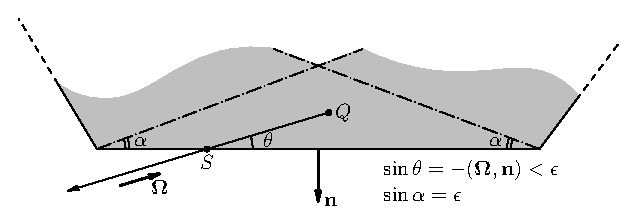
\includegraphics[width=.8\textwidth]{shift-0}
\caption{Точка $Q$ и выходящий из нее касательный луч. Точка $Q$ необходимо должна принадлежать 
серой области}
\label{fig:touch}
\end{figure}

Предположим, что грань является касательной к лучу. Это означает, что $\sin \theta = -(\vec \omega, 
\vec n) \leqslant \epsilon$. Поскольку обе точки $S,Q$ принадлежат $T$, то $|SQ| \leq d(T)$. 
Следовательно, высота, опущенная из $Q$ на грань $f$ не может иметь длину более $\sin \theta \cdot 
d(T) \leq \epsilon \cdot d(T) \equiv \delta$. Следовательно условие $\rho(Q, f) > \delta$ 
гарантирует, что луч не может выйти через грань $f$ так, чтобы быть к ней касательным. Обобщая это 
на все грани многогранника $T$, получаем утверждение леммы.
\end{proof}

Условие данной леммы можно усилить: $\rho(Q, f) > \delta$ является достаточным, но не необходимым. 
Однако, удовлетворить этому условию намного проще, чем точному условию (на рисунке
\ref{fig:forb} точное запрещенное множество закрашено серым цветом, а пунктиром обозначено множество из леммы).
\begin{figure}[ht!]
\centering
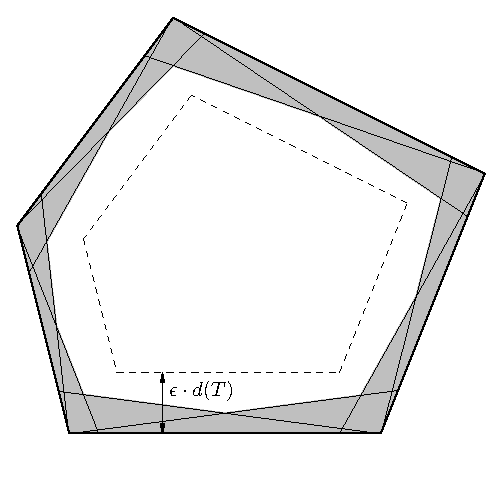
\includegraphics[width=.5\textwidth]{shift-1}%
\caption{Исходный многогранник, запрещенная область (серая) и область из леммы. Для трехмерного 
случая реальная запрещенная область имеет достаточно сложную форму}
\label{fig:forb}
\end{figure}

\begin{figure}[ht!]
\centering
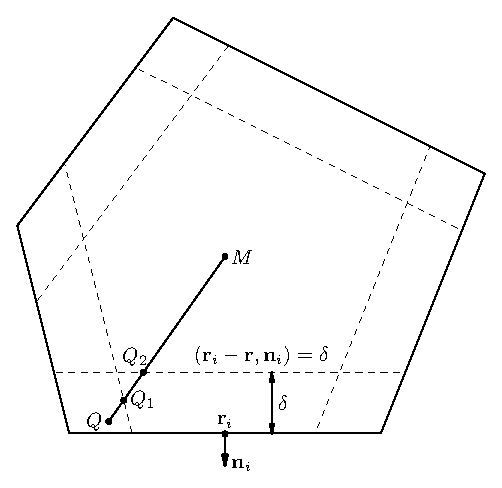
\includegraphics[width=.5\textwidth]{shift-2}%
\caption{Иллюстрация процедуры сдвига точки $Q$ в допустимое множество из леммы}
\end{figure}
Однако, простота этого условия порождает простую процедуру сдвига точки в допустимое множество (при 
условии, что центр масс $M$ многогранника сам лежит в допустимом множестве). Рассмотрим отрезок, 
соединяющий точки $M$ и $Q$, а также все плоскости, содержащие грани многогранника. Пусть каждая из 
этих плоскостей задана уравнением $(\vec r_i - \vec r, \vec n_i) = 0$. Несложно заметить, что 
условия леммы требуют выполнения соотношений $(\vec r_i - \vec r_Q, \vec n_i) > \delta$ для каждой 
$i$-й грани многогранника. Дополнительно требуя, чтобы новая точка $Q_i$ лежала на отрезке $QM$, 
получаем соотношения
\begin{gather*}
\vec r_{Q'} = \lambda \vec r_{Q} + (1 - \lambda) \vec r_{M}, \quad \lambda \in [0,1]\\
\lambda \rightarrow \max_{(\vec r_i - \vec r_{Q_i}, \vec n_i) > \delta}
\end{gather*}
Данная система линейных неравенств на $\lambda$ может быть легко решена последовательно для каждой грани, с выбором минимального $\lambda = \min_i \lambda_i$, см. алгоритм \ref{alg:shift}.

\begin{algorithm}[ht!]
\centering
\begin{algorithmic}[1]
\Function{ShiftToStable}{$e, Q$}
\State $\lambda := 1$
\State $\delta := \epsilon \cdot d(e)$
\State $\vec r_M := $ \Call{MassCenter}{$e$}
\For{каждой грани $f \in e$}
\State $(\vec r_i, \dots) := $ \Call{VertexCoordinates}{$f$}
\Comment Выбрать точку $\vec r_i \in f$
\State $\vec n_i := $ \Call{FaceNormal}{$f$}
\State $\vec r_{Q'} = \lambda \vec r_Q + (1 - \lambda) \vec r_{M}$
\If{$(\vec r_i - \vec r_{Q'}, \vec n_i) > \delta$}
\State \textbf{continue} \Comment Перейти к следующей грани
\Else
\State $\triangleright$ Найти точку пересечения отрезка $QM$ и плоскости
\State $\lambda := \frac{\delta - (\vec r_i - \vec r_M, \vec n_i)}
{(\vec r_Q - \vec r_M, \vec n_i)}$
\EndIf
\EndFor
\State $\vec r_{Q'} = \lambda \vec r_Q + (1 - \lambda) \vec r_{M}$
\State\Return{$Q'$}
\EndFunction
\end{algorithmic}
\caption{Алгоритм смещения точки в элементе}
\label{alg:shift}
\end{algorithm}

Заметим, что при использовании сдвига, длина отрезка характеристики в многограннике не меньше $\delta$, а следовательно при прохождении очередного тетраэдра точка продвигается в направлении $-\vec \Omega$ хотя бы на расстояние $\delta$.
Трассировка области с вычислением коэффициентов $\alpha, \beta$ представлена в алгоритме \ref{alg:tracedom}.

\begin{algorithm}[ht!]
\centering
\begin{algorithmic}[1]
\Function{TraceDomain}{$\mathcal{T}, P \in D, \vec\omega$}
\State $\alpha := 1$
\State $\beta := 0$
\State $e := $ \Call{ContainingElement}{$\mathcal{T}, P$}
\Repeat
\State $(Q, f. \ell, \vec\gamma) :=$ \Call{TraceElement}{$e, P, \vec \omega$}
\State $\Delta := \ell \varkappa(e) $
\Comment{Оптическая толщина элемента $e$}
\State $q := e^{-\Delta}$
\State $\beta := \beta + (1 - q)\alpha I_e(e)$
\State $\alpha := q\alpha$
\State $e := $ \Call{NeighbourOverFace}{$\mathcal{T}, e, f$}
\State $P := Q$
\Until{\textbf{not} \Call{IsValidElement}{$e$}}
\State\Return{$\alpha, \beta, \vec \gamma, f$}
\EndFunction
\end{algorithmic}
\caption{Алгоритм трассировки в триангуляции $\mathcal{T}$ области}
\label{alg:tracedom}
\end{algorithm}

\section{Распределенный метод}

Реализация метода длинных характеристик осложняется, если вычислительная область разбита на подобласти. Обычно каждая подобласть принадлежит своему вычислительному процессу и трассировка характеристики становится сложной коллективной операцией.

Заметим, что формула \eqref{eq:connection} позволяет не только вычислить неизвестное значение $I(s)$ через известное значение $I(s_0)$, но и просто связать
линейным соотношением два значения интенсивности в двух точках на одном луче.
Если интенсивность излучения каким-то образом оказалась известной на границе вычислительных подобластей, то трассировку лучей достаточно провести в каждой подобласти независимо от других. В этом случае точка $\vec r_0$ --- это точка, в которой характеристика пересекает границу \emph{подобласти}, а не всей вычислительной области (см. рис. \ref{fig:mcm}).

\begin{figure}[ht]
\centering
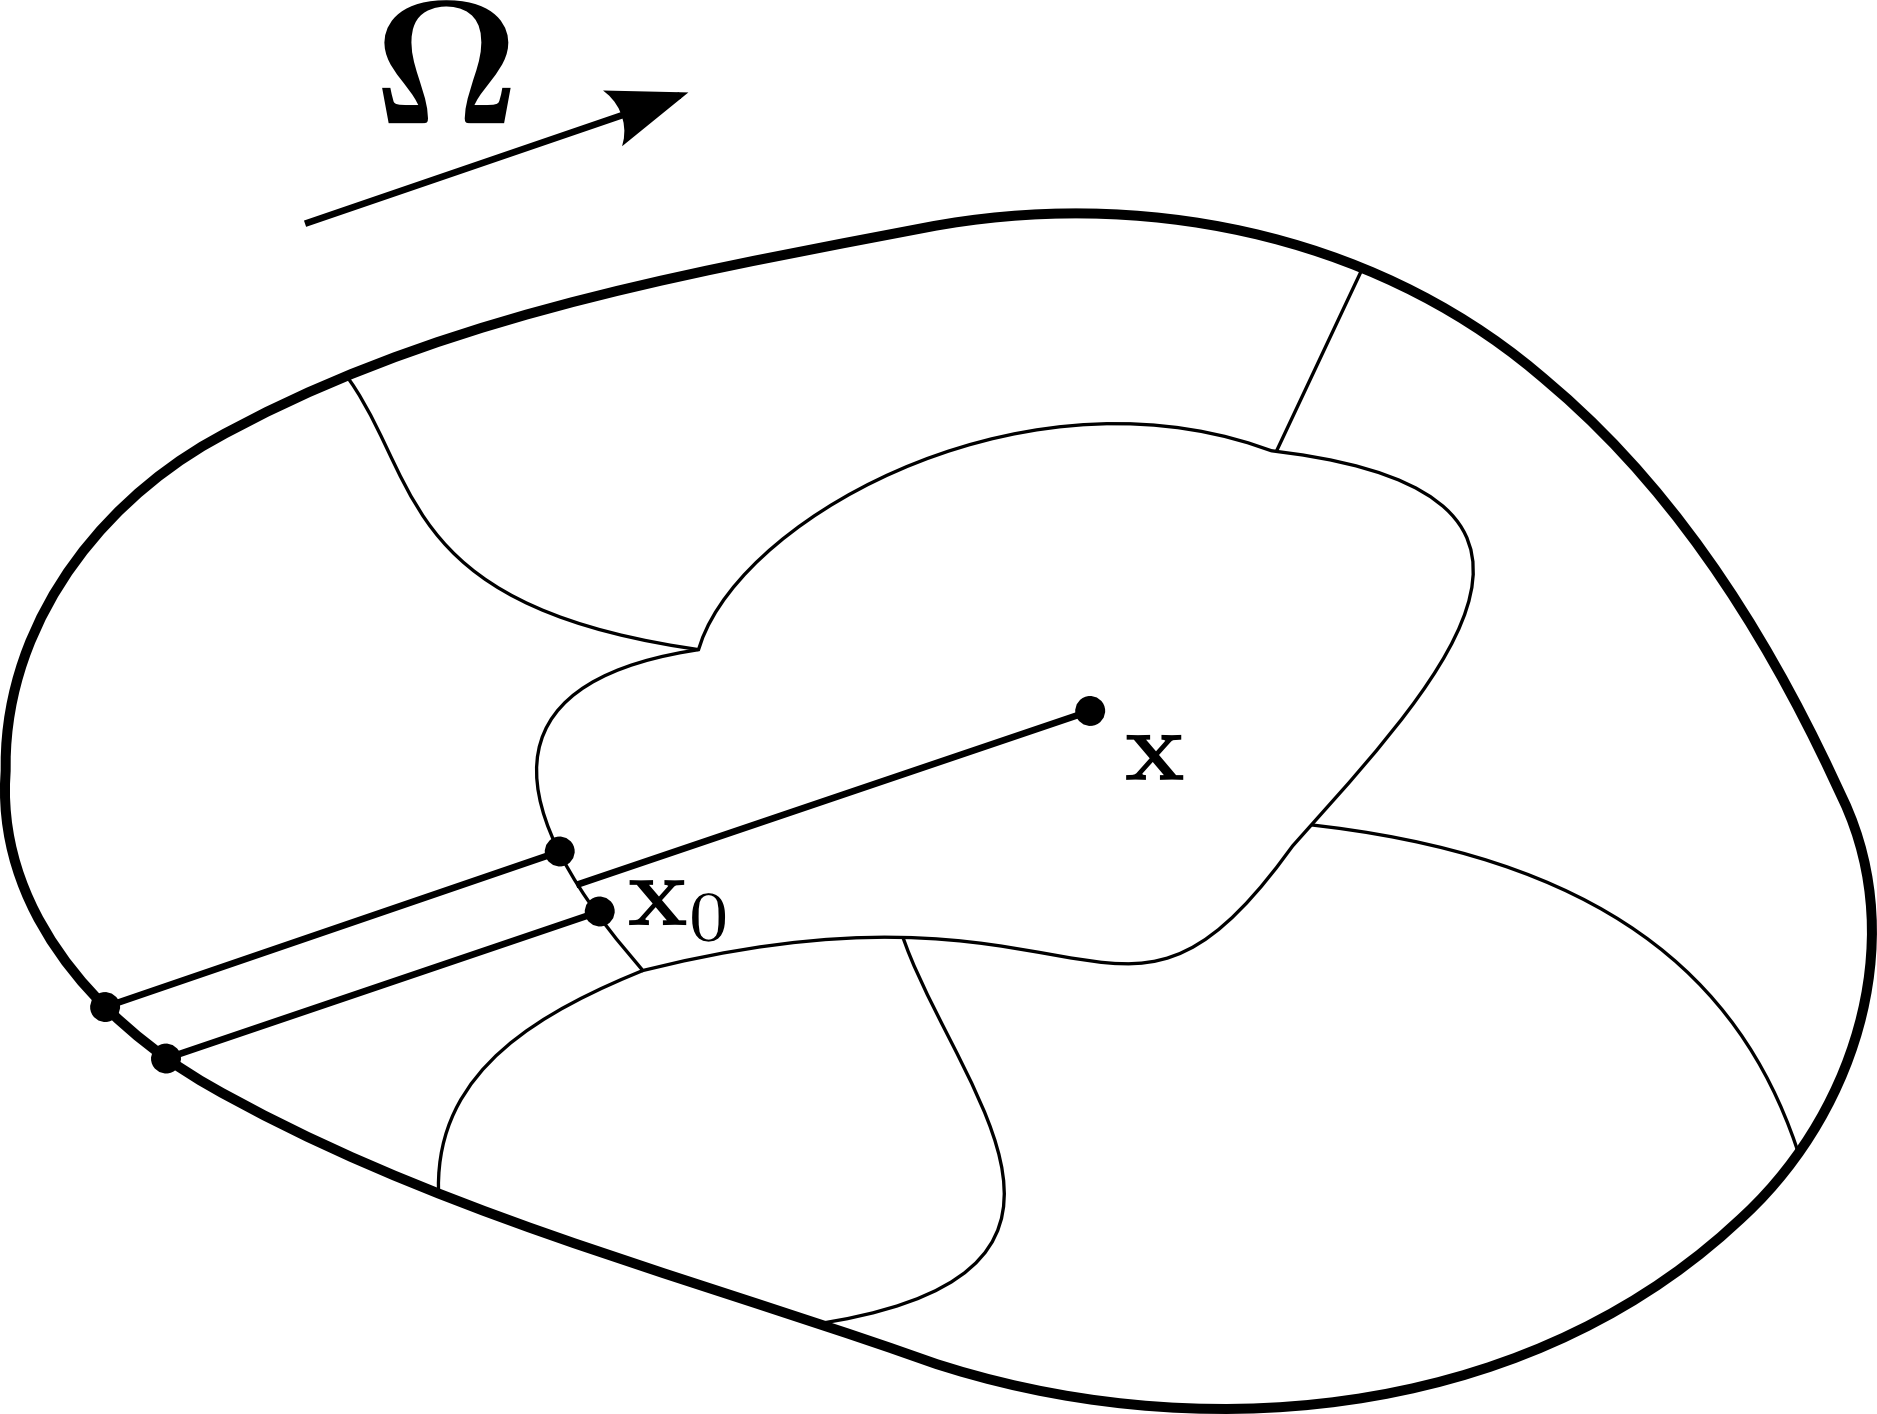
\includegraphics[height=0.3\textheight]{mcm.png}
\caption{Трассировка луча до границы подобласти}
\label{fig:mcm}
\end{figure}

Предположим, что границы подобластей проходят по граням тэтраэдральной сетки, построенной в области. Зафиксируем направление $\vec \Omega$. Будем говорить, что узел сетки (вершина тетраэдра) c координатой $\vec r$ принадлежит подобласти, если точка $\vec r - 0 \vec\Omega$ лежит в подобласти. Если таких подобластей несколько, например, если вектор $\vec \Omega$ лежит в плоскости грани, разделяющей подобласти, выберем подобласть с минимальным номером. Заметим, что определенное таким образом отношение принадлежности зависит не только от геометрических параметров сетки, но и от направления $\vec \Omega$ также. Если узел не принадлежит ни одной подобласти, будем говорить, что он принадлежит \emph{внешней} подобласти, то есть $\mathbb R^3 \setminus G$. Заметим, что интенсивность в граничных узлах, принадлежащих внешней подобласти задана граничными условиями.

Для каждого граничного узла с координатой $\vec r$, принадлежащего подобласти $D_i \subset G$ выпустим характеристику до пересечения с границей подобласти $\partial D_i$. В общем случае, характеристика выйдет из области через некоторую грань $f$ в точке $\vec r_0 = \vec r - \vec \Omega s$. 
Тогда пользуясь соотношением \eqref{eq:connection} заключаем, что
\[
I(\vec r) = \alpha(0, s) I(\vec r_0) + \beta(0, s).
\]
Однако, точка $\vec r$ является узлом расчетной сетки, а точка $\vec r_0$ в общем случае --- нет. Вычислим $I(\vec r_0)$ приближенно интерполяцией интенсивности по вершинам грани $f$
\[
I(\vec r_0) \approx \sum_{j=1}^F \gamma_j I(\vec r_j),
\]
где $F$ --- число вершин грани $f$ (для тетраэдральных сеток $F = 3$), а $\vec r_j$ --- координаты вершин этой грани, которые, в отличие от $\vec r_0$, являются узлами вычислительной сетки. Величины $\gamma_j$ являются обобщенными (для $F > 3$) барицентрическими координатами точки $\vec r_0$ в грани $f$. При этом $\sum_{j=1}^F \gamma_j = 1$.

Таким образом, получается система линейных уравнений, в которые входят значения интенсивности только на границах подобластей, и не входят значения внутри подобластей. Уравнения записаны для каждого граничного узла, принадлежащего некоторой вычислительной подобласти. В узлах, принадлежащих внешней подобласти интенсивность уже задана граничными условиями.

Отметим, что данная система уравнений имеет вид
\begin{equation}
I(\vec r) - \sum_{j=1}^K \gamma_j \alpha(0, s) I(\vec r_j) = \beta(0, s)
\label{eq:slae}
\end{equation}
и имеет диагональное преобладание, поскольку на диагонали стоит коэффициент $1$, а сумма модулей внедиагональных коэффициентов не превосходит $1 - \alpha(0, s) < 1$ некоторые из неизвестных $I(\vec r_j)$ могли быть исключены, если в $\vec r_j$ задано граничное условие).

После коллективного решения системы в узлах на границах подобластей становится известными значения интенсивности. Далее, выпуская характеристики из внутренних точек подобластей восстанавливается решение в каждом узле каждой подобласти всей расчетной области. Эта операция не является коллективной и проводится автономно в каждой подобласти. Также она является самой трудоемкой.

Необходимо подчеркнуть, что решение, полученное данным методом отличается от решения, полученного методом длинных характеристик. В частности, решение зависит от способа декомпозиции на подобласти. Предельный случай декомпозиции области на одну подобласть соответствует методу длинных характеристик, а гипотетический случай декомпозиции на отдельные тетраэдры приводит к методу, где характеристика выпускается от одной грани \emph{тетраэдра} до другой его грани, то есть интерполяция производится на каждой грани, а не только на границе подобласти, как в предлагаемом методе. При этом метод вырождается в метод коротких характеристик. Увеличение количества областей приводит к более частой интерполяции, которая, в свою очередь, вызывает численную диффузию луча. С другой стороны, при этом средняя длина трассируемых лучей уменьшается, что существенно снижает время работы алгоритма.

\section{Параллельная реализация вычислительного алгоритма}

Уравнение переноса решается в некотором наборе направлений. В качестве такого набора были выбраны узлы $\boldsymbol{\omega}_k$ квадратурной формулы для сферы Лебедева 

Для каждого направления $\vec \Omega$ граничные узлы каждой вычислительной подобласти разбиваются на те, которые ей принадлежат (в смысле определения, данного выше) и которые не принадлежат. Из тех, что принадлежат производится трассировка лучей вдоль направления $-\vec \Omega$ до пересечения с границей подобласти алгоритмом \ref{alg:tracedom}.

Таким образом, на каждый процесс формирует в своей подобласти часть общей системы уравнений, в которые входят неизвестные значения интенсивности на границе подобласти.
Далее эта система собирается воедино на одном из процессов, где решается прямым методом для разреженных матриц. Выбор такого метода вместо итерационного обусловлен двумя факторами. Во-первых, размер системы существенно меньше общего количества узлов сетки, так как неизвестные находятся лишь на границах подобластей. Во-вторых, матрицу системы можно превратить в близкую к треугольной, если упорядочить неизвестные по значению их проекции на луч $\vec \Omega$.

Чтобы эффективно использовать остальные процессы, пока на одном из них происходит решение системы, направления обрабатываются не по одному, а по несколько за раз. Это позволяет загрузить все процессы решением систем линейных уравнений, причем каждый процесс будет решать систему для своего направления.

Алгоритм решения состоит из следующих этапов:
\begin{enumerate}
\item Выбирается очередной набор направлений по одному на процесс.
\item Каждый процесс определяет принадлежащие ему точки и производит трассировку от границ в каждом направлении из набора.
\item На каждом процессе собирается система уравнений для его направления из набора.
\item Система решается на каждом процессе и полученное решение рассылается по всем процессам. После этого на каждом процессе становятся известны значения интенсивности на границе его подобласти.
\item В каждой подобласти производится вычисление решения во всех внутренних узлах автономно от остальных процессов.
\item Если остались направления, в которых решение еще не строилось, алгоритм повторяется с первого пункта.
\end{enumerate}

Так как пятый этап алгоритма самый трудоемкий, он был реализован с использованием графических ускорителей. Это позволило не только сократить время расчета задачи, но и произвести перекрытие подготовительных этапов (2-4), производимых на центральном процессоре с этапом 5, производимым на графическом ускорителе (см. рис. \ref{fig:timeline})
\begin{figure}[ht!]
\centering
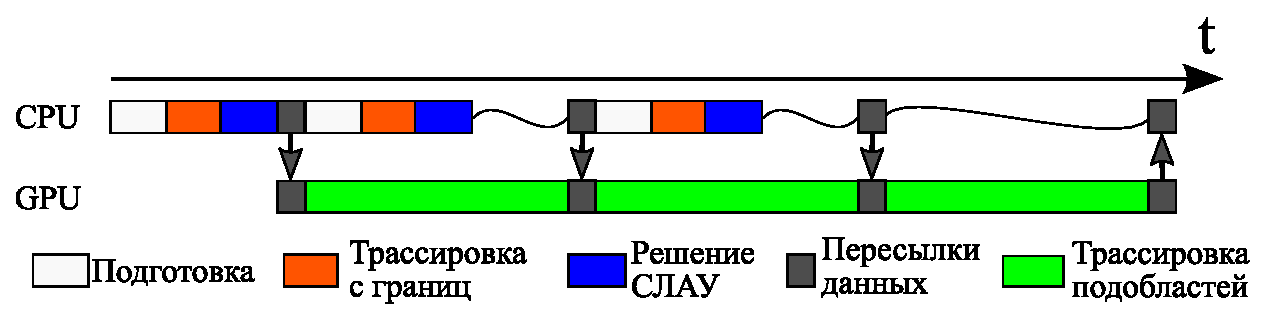
\includegraphics[width=0.8\linewidth]{timeline.eps}
\caption{Временная развертка алгоритма}
\label{fig:timeline}
\end{figure}
           % Глава 4
\chapter{Результаты}

Все численные методы были реализован в виде программ на языке C++ с использованием библиотеки CUDA \cite{cuda2015} для организации вычислений на графических процессорах. Использовались трехмерные сетки, сгенерированные программой NETGEN v4.9.14 \cite{Netgen2009}.
Для визуализации результатов применялась программа ParaView \cite{Paraview2004}.

\section{Исследование сходимости метода, основанного на вариационном принципе}

Тесты сходимости проводились на задаче об излучении оптически плотного излучающего шара радиуса $R = 0.3$ в поглощающей оптически менее плотной среде (см. приложение \ref{chap:problem}). Сравнивалась плотность энергии излучения. В окрестности поверхности шара плотность энергии имеет логарифмическую особенность производной, такую же, как и в задаче Милна (задача об излучении из полупространства).

Изучалась ошибка в точке $A(0, 0, 0)$ --- центре шара, $B\left(\frac{R}{\sqrt{3}}, \frac{R}{\sqrt{3}}, \frac{R}{\sqrt{3}}\right)$ --- точке на границе шара и в дискретной норме $L_2$:
\[
||u||_{DL_2} = \sqrt{\frac{1}{N}\sum_{i=1}^N u_i^2}
\]

Использовались пространственные сетки с количеством узлов от $7 \cdot 10^3$ до $206 \cdot 10^3$. Для метода сферических гармоник использовались сферические функции до $12$-й степени. Для метода радиальных базисных функций использовались $7$ первых квадратурных формул Лебедева в качестве сетки направлений. 

\subsection{Сходимость методов по количеству угловых функциях}

Анализ сходимости в дискретной норме $L_2$ показал, что зависимость ошибки на самой подробной сетке ($206 \cdot 10^3$ узлов) от числа используемых угловых функций $K$ носит одинаковый характер $\varepsilon \sim K^{-0.29}$, причем ошибка обоих методов практически одинакова при одинаковом количестве используемых угловых функций, см. график на рисунке \ref{fig:UL2err}.

\begin{figure}[ht!]
\centering
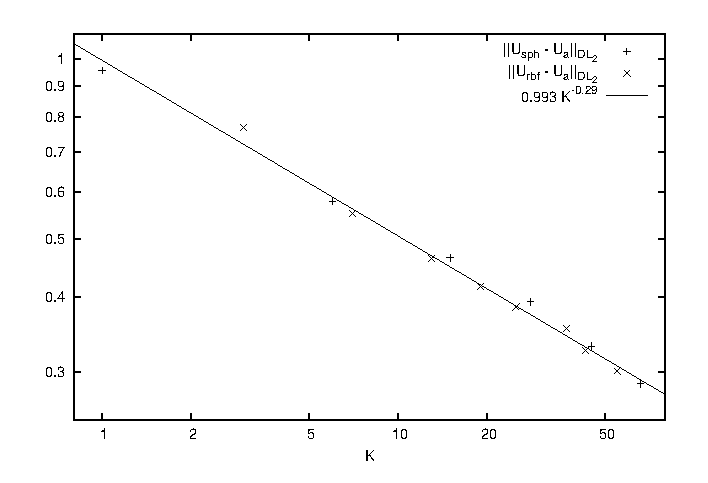
\includegraphics[width=\textwidth]{UL2err.eps}
\caption{Ошибка в норме $||\cdot||_{DL_2}$ в зависимости от числа угловых функций $K$}
\label{fig:UL2err}
\end{figure}

\subsection{Пространственная сходимость методов}

Сходимость методов изучалась в точке $A$ из области гладкости и в точке $B$ с границы шара при использовании самой подробной угловой дискретизации. Сходимость изучалась в зависимости от характерного шага сетки, принятого равным $N^{-1/3}$. На рисунке \ref{fig:UAerr} изображены графики ошибки в области гладкости и на границе шара.

\begin{figure}[ht!]
\centering
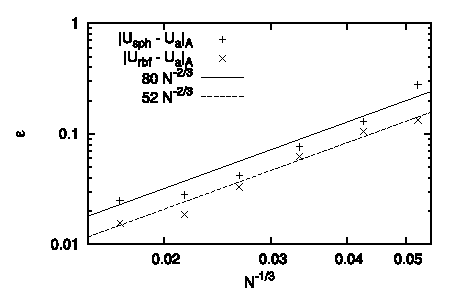
\includegraphics[width=.49\textwidth]{UAerr.eps}
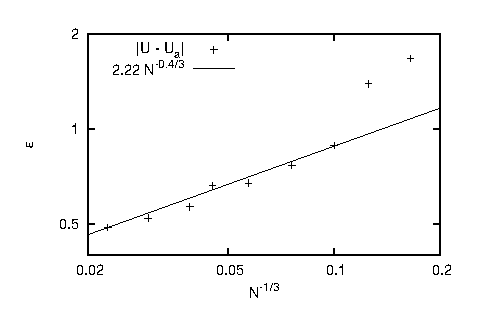
\includegraphics[width=.49\textwidth]{UBerr.eps}
\caption{Ошибка в точках $A, B$ в зависимости от характерного шага сетки $N^{-1/3}$}
\label{fig:UAerr}
\end{figure}

Порядок сходимости обоих методов в области гладкости равен двум. В области шара, где коэффициент поглощения меняется скачкообразно, порядок сходимости разный, он равен $\sim 0.4$ для метода сферических гармоник и $\sim 0.3$ для метода с радиальными базисными функциями, хотя разброс данных не позволяет достоверно определить порядок сходимости.

На рисунке \ref{fig:anvsnum} представлено решения вдоль оси $Ox$, полученные методом с радиальными функциями при $K = 55$ и методом сферических гармоник при $K = 91$. Видно, что существенное отличие численного решения от аналитического наблюдается в поглощающей области в окрестности шара.

Для обоих методов свойственны нефизичные значения интенсивности в области вдали от шара. Функция интенсивности, восстановленная из гармоник решения
\[
I(\vec r, \vec \Omega) = \sum_{k=1}^{n} I_k(\vec r) \theta_k (\vec \Omega)
\]
может содержать значения с отрицательными значениями интенсивности. В случае $I(\vec r, \vec \Omega) > 0$ тензор направленности излучения (тензор квазидиффузии) $\mathbb D$, определяемый как
\[
\mathbb D = \frac{\mathbb T}{U} = \frac{\int_{4\pi} \vec \Omega\vec \Omega I(\vec r, \vec \Omega) d\Omega}{\int_{4\pi} I(\vec r, \vec \Omega) d\Omega}
\]
имеет след, равный $1$ и неотрицательные компоненты. Однако, в численных расчетах свойство неотрицательности может нарушаться, если интенсивность $I(\vec r, \vec \Omega)$ принимает отрицательные значения (см. график на рисунке \ref{fig:Drad}). Значения $D_{rr} > 1$ свидетельствуют об отрицательности двух других главных компонент тензора $\mathbb D$.

\begin{figure}[ht!]
\centering
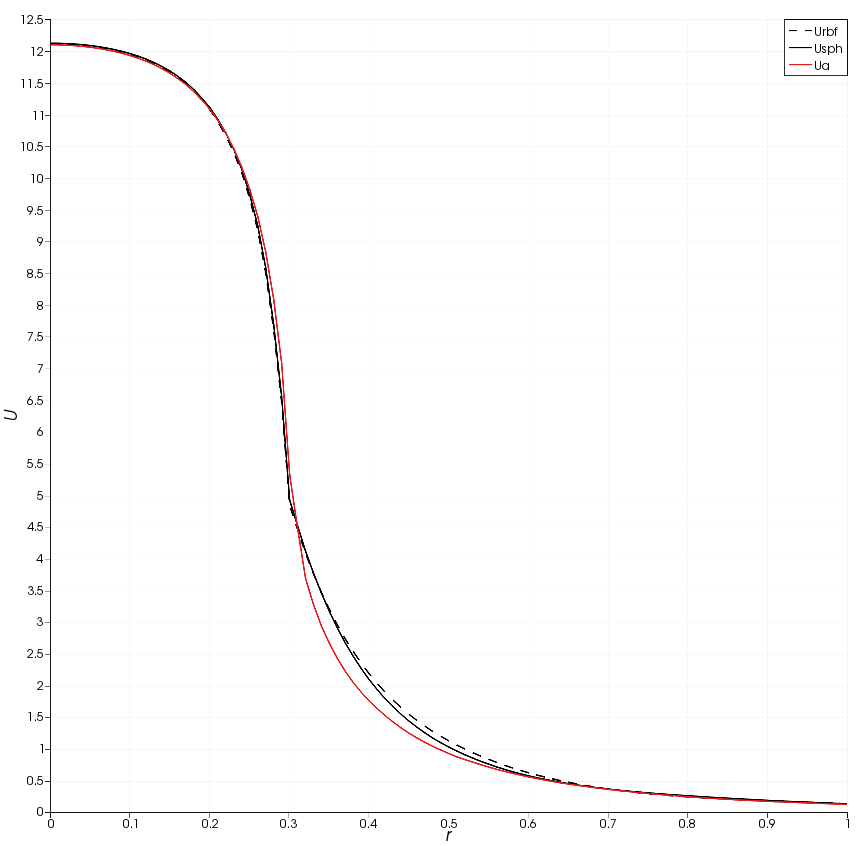
\includegraphics[width=.5\textwidth]{Uanvsnum.png}
\caption{Решения вдоль оси $Ox$, полученные методом с радиальными функциями при $K=55$ и методом сферических гармоник при $K = 91$}
\label{fig:anvsnum}
\end{figure}

\begin{figure}[ht!]
\centering
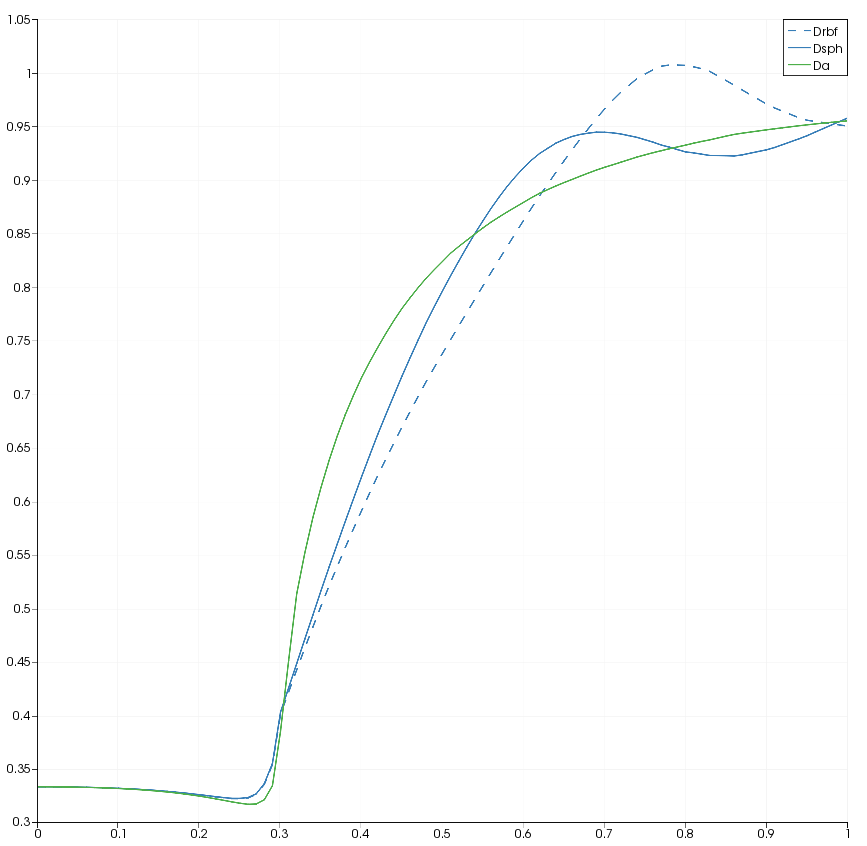
\includegraphics[width=.5\textwidth]{Dxx.png}
\caption{Радиальная компонента тензора направленноcти $\mathbb D_{rr}$ вдоль оси $Ox$}
\label{fig:Drad}
\end{figure}

Для исследования эффекта луча рассмотрим изоповерхности плотности интенсивности. Для метода сферических гармоник эффект луча отсутствует, поскольку базис из сферических функций инвариантен относительно произвольных вращений. На рисунке \ref{fig:iso} изображены изоповерхности решения построены для случая $K = 15$ метода сферических гармоник и $K = 13$ метода с радиальными функциями.

\begin{figure}[ht!]
\centering
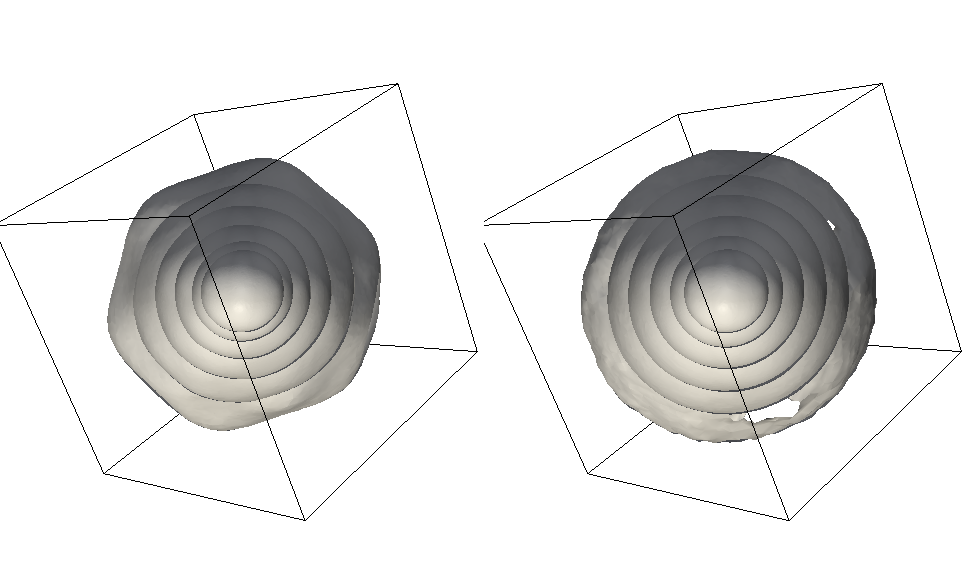
\includegraphics[width=\textwidth]{iso.png}
\caption{Изоповерхности плотности энергии излучения для метода с радиальными функциями (слева) и сферическими гармониками (справа)}
\label{fig:iso}
\end{figure}

\subsection{Сходимость метода при использовании предобуславливателя}

Для исследования сходимости внешних итераций метода сопряженных градиентов изучалось количество вызовов предобуславливателя для уменьшения нормы невязки в $10^{6}$ раз.

Отметим, что для метода сопряженных градиентов число итераций увеличивается как с увеличением количества угловых гармоник $K$, так и увеличением количества узлов сетки $N$. Для метода с радиальным базисом число итераций практически постоянно и равно $30$.

\begin{table}[ht!]
\RawFloats
\centering
\caption{Количество итераций метода сопряженных градиентов}
\begin{tabular}{cc|c|c|c|c|c|c|}
\cline{3-8}
& & \multicolumn{6}{|c|}{\rule{0em}{2.2ex}Количество узлов сетки} \\ \cline{3-8}
& & \rule{0em}{2.2ex}6996 & 12971 & 26786 & 53109 & 99015 & 205756\\ \cline{1-8}
\multicolumn{1}{|c|}{\multirow{7}{*}{\rotatebox{90}{Угловых  гармоник\phantom{x}}}} &
\multicolumn{1}{|c|}{\rule{0em}{2.2ex}1}  & 1 & 1 & 1 & 1 & 1 & 1 \\ 
\cline{2-8}\multicolumn{1}{|c|}{} &
\multicolumn{1}{|c|}{\rule{0em}{2.2ex}6}  & 20 & 21 & 22 & 23 & 25 & 26 \\ 
\cline{2-8}\multicolumn{1}{|c|}{} &
\multicolumn{1}{|c|}{\rule{0em}{2.2ex}15} & 29 & 31 & 33 & 34 & 37 & 38 \\ 
\cline{2-8}\multicolumn{1}{|c|}{} &
\multicolumn{1}{|c|}{\rule{0em}{2.2ex}28} & 36 & 38 & 41 & 44 & 48 & 51 \\ 
\cline{2-8}\multicolumn{1}{|c|}{} &
\multicolumn{1}{|c|}{\rule{0em}{2.2ex}45} & 42 & 45 & 49 & 53 & 57 & 62 \\ 
\cline{2-8}\multicolumn{1}{|c|}{} &
\multicolumn{1}{|c|}{\rule{0em}{2.2ex}66} & 46 & 50 & 55 & 60 & 65 & 70 \\ 
\cline{2-8}\multicolumn{1}{|c|}{} &
\multicolumn{1}{|c|}{\rule{0em}{2.2ex}91} & 48 & 53 & 59 & 65 & 71 & 77 \\ 
\cline{1-8}
\end{tabular}
\end{table}

\begin{table}[ht!]
\RawFloats
\centering
\caption{Количество итераций метода с радиальным базисом}
\begin{tabular}{cc|c|c|c|c|c|c|}
\cline{3-8}
& & \multicolumn{6}{|c|}{\rule{0em}{2.2ex}Количество узлов сетки} \\ \cline{3-8}
& & \rule{0em}{2.2ex}6996 & 12971 & 26786 & 53109 & 99015 & 205756\\ \cline{1-8}
\multicolumn{1}{|c|}{\multirow{7}{*}{\rotatebox{90}{Угловых гармоник\phantom{x}}}} &
\multicolumn{1}{|c|}{\rule{0em}{2.2ex}3}  & 13 & 14 & 15 & 14 & 15 & 15 \\ 
\cline{2-8}\multicolumn{1}{|c|}{} &
\multicolumn{1}{|c|}{\rule{0em}{2.2ex}7}  & 26 & 27 & 28 & 28 & 29 & 31 \\ 
\cline{2-8}\multicolumn{1}{|c|}{} &
\multicolumn{1}{|c|}{\rule{0em}{2.2ex}13} & 33 & 34 & 35 & 36 & 39 & 42 \\ 
\cline{2-8}\multicolumn{1}{|c|}{} &
\multicolumn{1}{|c|}{\rule{0em}{2.2ex}19} & 26 & 28 & 29 & 29 & 30 & 32 \\ 
\cline{2-8}\multicolumn{1}{|c|}{} &
\multicolumn{1}{|c|}{\rule{0em}{2.2ex}25} & 28 & 29 & 32 & 30 & 32 & 34 \\ 
\cline{2-8}\multicolumn{1}{|c|}{} &
\multicolumn{1}{|c|}{\rule{0em}{2.2ex}43} & 28 & 30 & 32 & 31 & 33 & 34 \\ 
\cline{2-8}\multicolumn{1}{|c|}{} &
\multicolumn{1}{|c|}{\rule{0em}{2.2ex}55} & 27 & 28 & 30 & 29 & 30 & 32 \\ 
\cline{1-8}
\end{tabular}
\end{table}

\section{Исследование маршевого метода коротких характеристик}

Для метода коротких характеристик изучалась численная диффузия луча. Центральное излучательное тело было заменено на крест, составленный из пяти одинаковых кубов (см. рисунок \ref{fig:cross}). Решение строилось для одного направления, при этом аналитическое решение представляет собой проекцию креста на грань тетраэдра. Оптическая толщина креста много больше единицы, а оптическая толщина окружающего пространства много меньше единицы. В таких условиях, решение на грани имеет интенсивность равную равновесной интенсивности в кресте.
\begin{figure}[ht!]
\centering
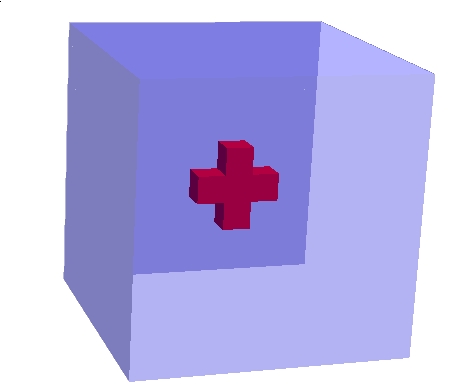
\includegraphics[width=.5\textwidth]{plus.png}
\caption{Вид излучающего тела для метода коротких характеристик}
\label{fig:cross}
\end{figure}

%\subsection{Сравнение численной диффузии луча в методах первого и второго порядка}

Для метода первого порядка решение на грани испытывает значительную диффузию. Для метода второго порядка без ограничителя решение нарушает принцип максимума. Отклонения интенсивности на грани от диапазона $[0, 1]$ составляет $20 \%$ (области на границе креста). Метод с ограничителем имеет решение, в котором принцип максимума не нарушен, а численная диффузия луча значительно меньше, чем в случае метода первого порядка.

\begin{figure}[ht!]
\centering
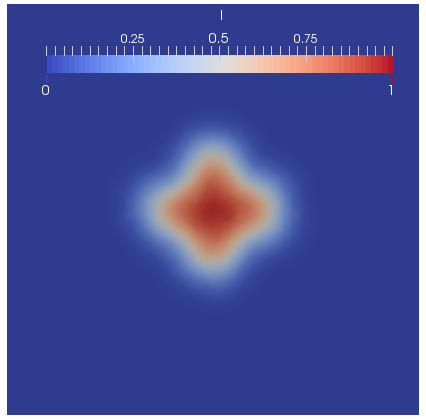
\includegraphics[width=.3\textwidth]{res1ord.png}
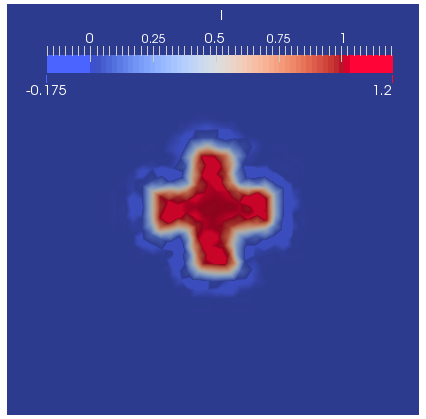
\includegraphics[width=.3\textwidth]{res2nolim.png}
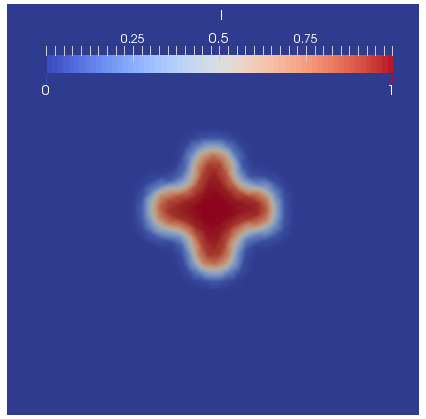
\includegraphics[width=.3\textwidth]{res2wilim.png}
\caption{Решение на грани для метода первого порядка (слева), метода второго порядка (в центре) и метода второго порядка с ограничителем (справа)}
\label{fig:limiter}
\end{figure}

Сравнение плотности излучения в решениях, полученных методом первого и второго порядка с ограничителем показывает близкие (в пределах $2\%$) решения (см графики на рисунках \ref{fig:U2vs1} и \ref{fig:U2vs1Line}). При этом для метода второго порядка плотность энергии излучения сосредоточена в кресте, в то время как в методе первого порядка она диффундирует за его пределы. К тому же, в методе второго порядка более выражен эффект луча, в методе же первого порядка, он сглажен численной диффузией.

\begin{figure}[ht!]
\centering
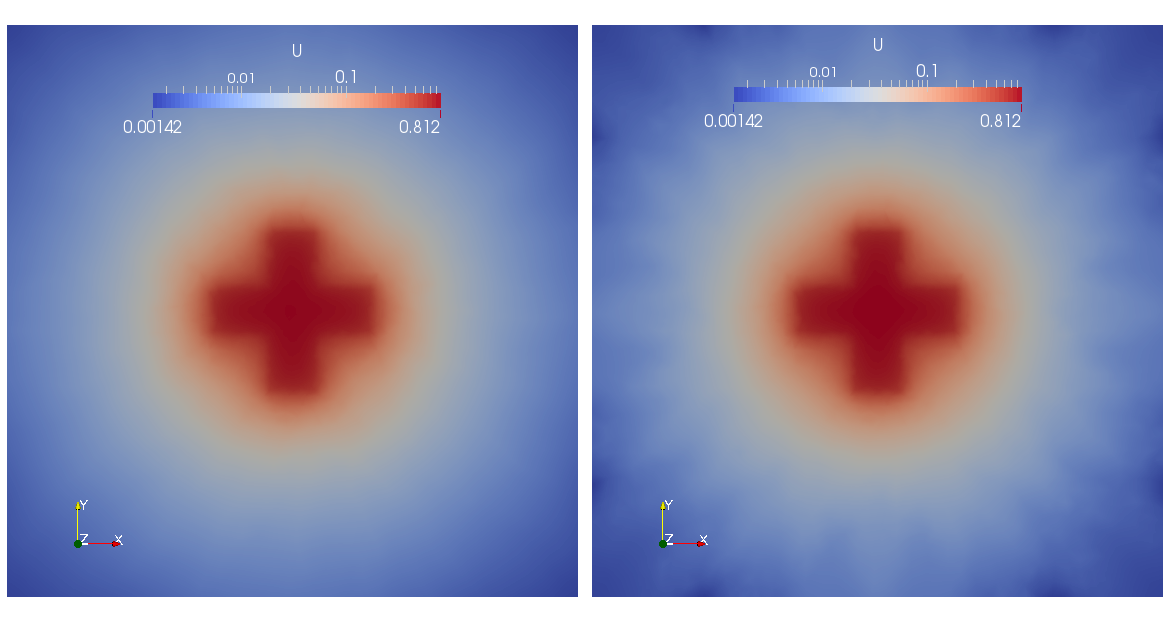
\includegraphics[height=.3\textheight]{U2vs1.png}
\caption{Плотность излучения в методе первого порядка (слева) и второго порядка с ограничителем (справа) в центральном сечении}
\label{fig:U2vs1}
\end{figure}

\begin{figure}[ht!]
\centering
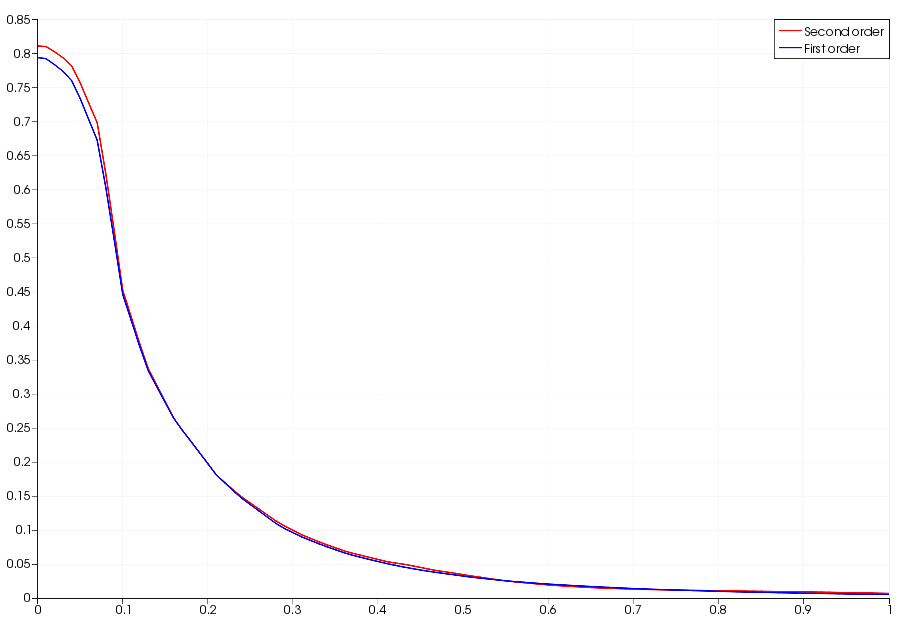
\includegraphics[height=.3\textheight]{U2vs1Line.png}
\caption{Плотность излучения в методе первого порядка (синий график) и второго порядка с ограничителем (красный график) вдоль луча, перпендикулярного кресту}
\label{fig:U2vs1Line}
\end{figure}

Дополнительно был рассмотрен метод первого порядка с увеличенным количеством узлов. В этом методе вместо квадратичной интерполяции по шести узлам используется кусочно-линейная. Данная операция позволяет сравнивать методы при одинаковом числе используемых узлов. Область и излучающее тело были заменены на концентрические шары, а поглощение в области отсутствовало. Диффузия луча носит качественно различный характер: в методе первого порядка диффузия луча имеет характер $\sim \sqrt{x}$, а в методе второго порядка диффузия луча практически постоянна вдоль луча.

\begin{figure}[ht!]
\centering
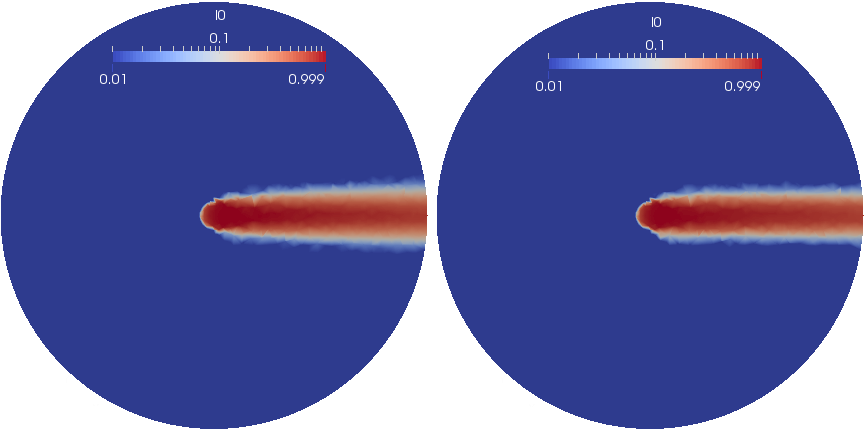
\includegraphics[width=\textwidth]{diff.png}
\caption{Диффузия луча в методе первого порядка с увеличенным числом узлов (слева) и методе второго порядка с ограничителем}
\label{fig:diff}
\end{figure}

\section{Исследование распределенного метода длинных характеристик}

\subsection{Сравнение решений для различного числа подобластей}

Для нескольких подобластей наблюдается незначительная диффузия луча, проходящего через границу подобластей.

\subsection{Ускорение и эффективность параллельной реализации}

Версия, использующая графические ускорители в $3.5$ раз быстрее версии для центрального процессора.

\section{Расчет спектра излучения линии H-$\alpha$ звезды типа Т Тельца}

\section{Выводы}
           % Глава 5
\chapter*{Заключение}						% Заголовок
\addcontentsline{toc}{chapter}{Заключение}	% Добавляем его в оглавление

%% Согласно ГОСТ Р 7.0.11-2011:
%% 5.3.3 В заключении диссертации излагают итоги выполненного исследования, рекомендации, перспективы дальнейшей разработки темы.
%% 9.2.3 В заключении автореферата диссертации излагают итоги данного исследования, рекомендации и перспективы дальнейшей разработки темы.
%% Поэтому имеет смысл сделать эту часть общей и загрузить из одного файла в автореферат и в диссертацию:

Основные результаты работы:
%% Согласно ГОСТ Р 7.0.11-2011:
%% 5.3.3 В заключении диссертации излагают итоги выполненного исследования, рекомендации, перспективы дальнейшей разработки темы.
%% 9.2.3 В заключении автореферата диссертации излагают итоги данного исследования, рекомендации и перспективы дальнейшей разработки темы.
\begin{enumerate}
  \item Для решения уравнения переноса излучения разработан вариационный метод с радиальными базисными функциями, который обладает точностью, сравнимой с методом сферических гармоник, но при этом более экономичный. Предложенное блочно-диагональное предобуславливание позволяет значительно ускорить вычислительный алгоритм. Построены оптимальные квадратурные формулы для полусферы, инвариантные относительно группы вращений.
  \item Разработан маршевый метод коротких характеристик. Построены варианты метода первого и второго порядка аппроксимации. Получено условие расположения узлов, выполнение которого необходимо для устойчивости метода второго порядка. Для монотонизации схемы второго порядка применен ограничитель значения интенсивности в дополнительных узлах.
  \item Для маршевого метода построены алгоритмы упорядочения неструктурированных сеток. Дополнительным результатом работы алгоритмов упорядочения является ярусно-параллельная форма графа зависимостей вычислительного метода, которую можно использовать для распараллеливания процесса решения задачи. 
  \item Разработана версия метода длинных характеристик, адаптированная для распределенной реализации на многопроцессорных системах и на кластерах с графическими ускорителями. Исследованы ускорение и эффективность реализаций в зависимости от числа используемых вычислительных узлов и графических ускорителей.
  \item Разработанные вычислительные алгоритмы реализованы в программном комплексе. В рамках модели локального термодинамического равновесия вычислен коэффициент поглощения частично ионизованной плазмы. Для задачи моделирования спектра излучения звезды типа Т Тельца построен спектральный профиль линии H-$\alpha$ в зависимости от ориентации плоскости аккреционного диска.
\end{enumerate}


%\todo{Разбавить словами}
      % Заключение
\clearpage                                  % В том числе гарантирует, что список литературы в оглавлении будет с правильным номером страницы
\phantomsection
\addcontentsline{toc}{chapter}{\bibname}	% Добавляем список литературы в оглавление
%\hypersetup{ urlcolor=black }               % Ссылки делаем чёрными
%\providecommand*{\BibDash}{}                % В стилях ugost2008 отключаем использование тире как разделителя 
\urlstyle{rm}                               % ссылки URL обычным шрифтом
\insertbibliofull                          % Подключаем Bib-базы
\urlstyle{tt}                               % возвращаем установки шрифта ссылок URL
%\hypersetup{ urlcolor={urlcolor} }          % Восстанавливаем цвет ссылок
      % Список литературы
\appendix
%% Правка оформления ссылок на приложения:
%http://tex.stackexchange.com/questions/56839/chaptername-is-used-even-for-appendix-chapters-in-toc
%http://tex.stackexchange.com/questions/59349/table-of-contents-with-chapter-and-appendix
%% требует двойной компиляции
\addtocontents{toc}{\def\protect\cftchappresnum{\appendixname{} }%
\setlength{\cftchapnumwidth}{\widthof{\cftchapfont\appendixname~Ш\cftchapaftersnum}}%
}
%% Оформление заголовков приложений ближе к ГОСТ:
\sectionformat{\chapter}[display]{% Параметры заголовков разделов в тексте
    label=\chaptertitlename\ \thechapter,% (ГОСТ Р 2.105, 4.3.6)
    labelsep=20pt,
}
\renewcommand\thechapter{\Asbuk{chapter}} % Чтобы приложения русскими буквами нумеровались
\chapter{прила}       % Приложения 
\chapter{Сферические функции}
\label{chap:spher}

\section{Сферические функции, используемые в работе}

В работе были использованы действительные сферические функции, образующие ортонормированную систему по отношению
к скалярному произведению $(\varphi, \psi) = \frac{1}{4\pi} \int \varphi \psi d\Omega$. Они имеют следующее представление
\begin{align*}
Y_{l,m}(\theta, \varphi) &= C_{l,m}P_l^{m}(\cos \theta)\times
\begin{cases}
\sin |m| \varphi,&\, m<0\\
\frac{1}{\sqrt{2}},&\, m=0\\
\cos m \varphi,&\, m>0\\
\end{cases}
\label{eq:sphfunc}\\
C_{l,m} &= (-1)^{\frac{|m|+m}{2}}\sqrt{4l+2}\sqrt{\frac{(l-m)!}{(l+m)!}},
\end{align*}
где $P^m_l(\mu)$ --- присоединенный многочлен Лежандра степени $l$ и порядка $m$.

Сферические функции могут быть выражены как однородные многочлены от компонент $\vec \Omega$. Представление нескольких первых 
функций приведено ниже:
\begin{align*}
Y_{0,0} &= 1\\
Y_{1,-1} = \sqrt{3}\Omega_y,\quad
Y_{1,0} &= \sqrt{3}\Omega_z,\quad
Y_{1,1} = \sqrt{3}\Omega_x\\
Y_{2,-2} = \sqrt{15}\Omega_x\Omega_y,\quad
Y_{2,-1} &= \sqrt{15}\Omega_y\Omega_z, \quad
Y_{2,1} = \sqrt{15}\Omega_x\Omega_z\\
Y_{2,0} = \sqrt{5}\Omega_z^{2}&-\frac{\sqrt{5}}{2}\Omega_y^{2}-\frac{\sqrt{5}}{2}\Omega_x^{2}\\
Y_{2,2} = \frac{\sqrt{15}}{2}\Omega_x^{2}&-\frac{\sqrt{15}}{2}\Omega_y^{2}
\end{align*}

\section{Правила отбора для интеграла от трех действительных сферических функций}

Рассмотрим следующий интеграл
\[
\begin{bmatrix}
l_1 & l_2 & l_3\\
m_1 & m_2 & m_3
\end{bmatrix} \equiv
\int\limits_{4\pi}
Y_{l_1,m_1}(\vec \Omega)
Y_{l_2,m_2}(\vec \Omega)
Y_{l_3,m_3}(\vec \Omega)
d\Omega.
\]
Без ограничений общности, предположим, что $l_1 \leq l_2 \leq l_3$.
Найдем необходимые условия, при которых он отличен от нуля. Учтем, что сферические функции допускают представление
\[
Y_{l,m}(\vec \Omega) = C_{l,m} P_l^{m}(\cos \theta) \Phi_m(\varphi),
\]
а, следовательно, рассматриваемый интеграл может быть записан как
\begin{multline*}
\begin{bmatrix}
l_1 & l_2 & l_3\\
m_1 & m_2 & m_3
\end{bmatrix} =
C_{l_1,m_1}
C_{l_2,m_2}
C_{l_3,m_3} \times \\ \times
\int\limits_{-1}^1 
P_{l_1}^{m_1}(\mu)
P_{l_2}^{m_2}(\mu)
P_{l_3}^{m_3}(\mu)
d\mu
\int\limits_{0}^{2\pi}
\Phi_{m_1}(\varphi)
\Phi_{m_2}(\varphi)
\Phi_{m_3}(\varphi)
d\varphi
\end{multline*}
Для интеграла
\[
\int\limits_{-1}^1 
P_{l_1}^{m_1}(\mu)
P_{l_2}^{m_2}(\mu)
P_{l_3}^{m_3}(\mu)
d\mu
\]
известны \cite{Gaunt1929} правила отбора, которые заключаются в том, что интеграл не равен нулю только если выполнены следующие предположения:
\begin{itemize}
\item сумма степеней $l_1 + l_2 + l_3$ четна;
\item степени удовлетворяют неравенству треугольника $l_3 < l_1 + l_2$.
\end{itemize}

Для интеграла 
\[
\int\limits_{0}^{2\pi}
\Phi_{m_1}(\varphi)
\Phi_{m_2}(\varphi)
\Phi_{m_3}(\varphi)
d\varphi
\]
рассмотрим возможные случаи.
\paragraph{Случай $m_1 = 0$.} Поскольку $\Phi_0(\varphi) = \frac{1}{\sqrt{2}}$, интеграл сводится к 
\[
\int\limits_{0}^{2\pi}
\Phi_{m_2}(\varphi)
\Phi_{m_3}(\varphi)
d\varphi,
\]
который отличен от нуля только при $m_2 = m_3$.
\paragraph{Случай $m_1 \leq m_2 \leq m_3 < 0$.} Интеграл представим в виде
\begin{multline*}
-\int\limits_{0}^{2\pi}
\sin m_1 \varphi
\sin m_2 \varphi
\sin m_3 \varphi
d\varphi = \\ 
= 
\frac{1}{2}\int\limits_{0}^{2\pi}
\sin m_1 \varphi
\cos (m_2 + m_3) \varphi
d\varphi 
-
\frac{1}{2}\int\limits_{0}^{2\pi}
\sin m_1 \varphi
\cos (m_3 - m_2) \varphi
d\varphi.
\end{multline*}
Оба интеграла равны нулю. 

\paragraph{Случай $m_1 \leq m_2 < 0 < m_3$.} Интеграл представим в виде
\begin{multline*}
\int\limits_{0}^{2\pi}
\sin m_1 \varphi
\sin m_2 \varphi
\cos m_3 \varphi
d\varphi = \\ 
= 
\frac{1}{2}\int\limits_{0}^{2\pi}
\cos (m_2 - m_1) \varphi
\cos m_3 \varphi
d\varphi 
+
\frac{1}{2}\int\limits_{0}^{2\pi}
\cos (m_1 + m_2) \varphi
\cos m_3 \varphi
d\varphi.
\end{multline*}
Интеграл отличен от нуля если $m_3 = m_2 - m_1$ либо $m_3 = -m_1 - m_2$.

\paragraph{Случай $m_1 < 0 < m_2 \leq m_3$.} Интеграл представим в виде
\begin{multline*}
-\int\limits_{0}^{2\pi}
\sin m_1 \varphi
\cos m_2 \varphi
\cos m_3 \varphi
d\varphi = \\ 
= 
-\frac{1}{2}\int\limits_{0}^{2\pi}
\sin m_1 \varphi
\cos (m_2 + m_3) \varphi
d\varphi 
-
\frac{1}{2}\int\limits_{0}^{2\pi}
\sin m_1 \varphi
\cos (m_2 - m_3) \varphi
d\varphi.
\end{multline*}
Оба интеграла равны нулю. 

\paragraph{Случай $0 < m_1 \leq m_2 \leq m_3$.} Интеграл представим в виде
\begin{multline*}
\int\limits_{0}^{2\pi}
\cos m_1 \varphi
\cos m_2 \varphi
\cos m_3 \varphi
d\varphi = \\ 
= 
\frac{1}{2}\int\limits_{0}^{2\pi}
\cos m_1 \varphi
\cos (m_2 + m_3) \varphi
d\varphi 
+
\frac{1}{2}\int\limits_{0}^{2\pi}
\cos m_1 \varphi
\cos (m_2 - m_3) \varphi
d\varphi.
\end{multline*}
Интеграл отличен от нуля только если $m_1 + m_2 = m_3$ (случай $m_1 = m_2 + m_3$ невозможен, т.к. $m_3 \geq m_1, m_2 > 0$).

Подытожим, интеграл 
\[
\int\limits_{0}^{2\pi} \Phi_{m_1}(\varphi)\Phi_{m_2}(\varphi)\Phi_{m_3}(\varphi) d\varphi, \quad 
m_1 \leq m_2 \leq m_3,
\]
отличен от нуля только если
\begin{itemize}
\item одно из чисел $m_1, m_2, m_3$ равно нулю, а остальные равны между собой;
\item либо $m_1, m_2, m_3 > 0$ и $m_3 = m_1 + m_2$;
\item либо $m_1, m_2 < 0, m_3 > 0$, при этом либо $m_1 + m_2 + m_3 = 0$, либо $m_1 - m_2 + m_3 = 0$.
\end{itemize}
В совокупности с правилами отбора для степеней $l_1, l_2, l_3$
\begin{itemize}
\item сумма степеней $l_1 + l_2 + l_3$ четна;
\item степени удовлетворяют неравенству треугольника $l_3 < l_1 + l_2$,
\end{itemize}
эти требования составляют правила отбора для интеграла
\[
\begin{bmatrix}
l_1 & l_2 & l_3\\
m_1 & m_2 & m_3
\end{bmatrix} \equiv
\int\limits_{4\pi}
Y_{l_1,m_1}(\vec \Omega)
Y_{l_2,m_2}(\vec \Omega)
Y_{l_3,m_3}(\vec \Omega)
d\Omega.
\]

\section{Матрица
\texorpdfstring{$\mathscr{K}^{\alpha\beta}_{kk'}$}{K^ab\_kk'}
приближения \texorpdfstring{$n = 1$}{n = 1}}

Для иллюстрации разреженной структуры матрицы, приведен вариант при $n = 2$. Блоки соответствуют следующей нумерации сферических гармоник: 
$\varphi_{0,0}\quad \varphi_{2,-2}\quad \varphi_{2,-1}\quad \varphi_{2,0}\quad \varphi_{2,1}\quad \varphi_{2,2}$

\begin{small}
\begin{align*}
%&\langle \Omega_i \Omega_j \rangle_{2k\,m}^{2k'\,m'} = \\
%&
\left(
\begin{array}{@{}c@{}c@{}c||c@{}cc|cc@{}c|c@{}c@{}c|ccc|@{}c@{}c@{}c@{}}
\frac{1}{3}&0&0&
0&\frac{\sqrt{15}}{15}&0&
0&0&0&
-\frac{\sqrt{5}}{15}&0&0&
0&0&\frac{\sqrt{15}}{15}&
\frac{\sqrt{15}}{15}&0&0\\
0&\frac{1}{3}&0&
\frac{\sqrt{15}}{15}&0&0&
0&0&\frac{\sqrt{15}}{15}&
0&-\frac{\sqrt{5}}{15}&0&
0&0&0&
0&-\frac{\sqrt{15}}{15}&0\\
0&0&\frac{1}{3}&
0&0&0&
0&\frac{\sqrt{15}}{15}&0&
0&0&\frac{2\sqrt{5}}{15}&
\frac{\sqrt{15}}{15}&0&0&
0&0&0\\
\hline
\hline
0&\frac{\sqrt{15}}{15}&0&
\frac{3}{7}&0&0&
0&0&\frac{1}{7}&
0&-\frac{2\sqrt{3}}{21}&0&
0&0&0&
0&0&0\\
\frac{\sqrt{15}}{15}&0&0&
0&\frac{3}{7}&0&
0&0&0&
-\frac{2\sqrt{3}}{21}&0&0&
0&0&\frac{1}{7}&
0&0&0\\
0&0&0&
0&0&\frac{1}{7}&
\frac{1}{7}&0&0&
0&0&0&
0&\frac{1}{7}&0&
0&0&0\\
\hline
0&0&0&
0&0&\frac{1}{7}&
\frac{1}{7}&0&0&
0&0&0&
0&\frac{1}{7}&0&
0&0&0\\
0&0&\frac{\sqrt{15}}{15}&
0&0&0&
0&\frac{3}{7}&0&
0&0&\frac{\sqrt{3}}{21}&
\frac{1}{7}&0&0&
0&0&-\frac{1}{7}\\
0&\frac{\sqrt{15}}{15}&0&
\frac{1}{7}&0&0&
0&0&\frac{3}{7}&
0&\frac{\sqrt{3}}{21}&0&
0&0&0&
0&-\frac{1}{7}&0\\
\hline
-\frac{\sqrt{5}}{15}&0&0&
0&-\frac{2\sqrt{3}}{21}&0&
0&0&0&
\frac{5}{21}&0&0&
0&0&\frac{\sqrt{3}}{21}&
-\frac{2\sqrt{3}}{21}&0&0\\
0&-\frac{\sqrt{5}}{15}&0&
-\frac{2\sqrt{3}}{21}&0&0&
0&0&\frac{\sqrt{3}}{21}&
0&\frac{5}{21}&0&
0&0&0&
0&\frac{2\sqrt{3}}{21}&0\\
0&0&\frac{2\sqrt{5}}{15}&
0&0&0&
0&\frac{\sqrt{3}}{21}&0&
0&0&\frac{11}{21}&
\frac{\sqrt{3}}{21}&0&0&
0&0&0\\
\hline
0&0&\frac{\sqrt{15}}{15}&
0&0&0&
0&\frac{1}{7}&0&
0&0&\frac{\sqrt{3}}{21}&
\frac{3}{7}&0&0&
0&0&\frac{1}{7}\\
0&0&0&
0&0&\frac{1}{7}&
\frac{1}{7}&0&0&
0&0&0&
0&\frac{1}{7}&0&
0&0&0\\
\frac{\sqrt{15}}{15}&0&0&
0&\frac{1}{7}&0&
0&0&0&
\frac{\sqrt{3}}{21}&0&0&
0&0&\frac{3}{7}&
\frac{1}{7}&0&0\\
\hline
\frac{\sqrt{15}}{15}&0&0&
0&0&0&
0&0&0&
-\frac{2\sqrt{3}}{21}&0&0&
0&0&\frac{1}{7}&
\frac{3}{7}&0&0\\
0&-\frac{\sqrt{15}}{15}&0&
0&0&0&
0&0&-\frac{1}{7}&
0&\frac{2\sqrt{3}}{21}&0&
0&0&0&
0&\frac{3}{7}&0\\
0&0&0&
0&0&0&
0&-\frac{1}{7}&0&
0&0&0&
\frac{1}{7}&0&0&
0&0&\frac{1}{7}
\end{array}
\right)
\end{align*}
\end{small}       % Приложения 

\end{document}
